\documentclass[11pt,twoside,a4paper]{book}
% Pour avoir les lettres accentu�es  et l'hyph�nation
\usepackage[T1, T5]{fontenc}
\usepackage{lmodern}
\usepackage[applemac]{inputenc}
\usepackage[english]{babel}



\usepackage{epsfig}
\usepackage{mathrsfs}
\usepackage{color}
\usepackage{amsthm}
\usepackage{amsmath}
\usepackage{amsfonts}
\usepackage{amssymb}
%\usepackage{showkeys}
\usepackage{graphicx}
\usepackage{graphics}
\usepackage{subfigure}

\usepackage{import} % pour les .pdf_tex

\usepackage{pdfsync}


\usepackage{fullpage}
\usepackage{xspace}
%\usepackage[table]{xcolor}

\usepackage{minitoc} % pour la table des matieres � chaque chapitre


%%% FOOTNOTE
%\usepackage{footnpag}
\usepackage{footmisc}

%% Mes macros � moi
\usepackage{MesCommandes}


%% HYPERREF (pdf interactif) A PLACER EN DERNIER !!!
\usepackage[pdftex]{hyperref}


\newcommand{\code}[1]{\texttt{#1}}


\title{$\mu$-diff Matlab toolbox: user guide}

%\author{X. Antoine\thanks{Institut Elie Cartan Nancy (IECN), Nancy University, INRIA Corida Team, B.P. 239, F-54506
%    Vandoeuvre-l\`es-Nancy Cedex, France.}, \and
%  C. Besse\thanks{?} \and P. Klein}

\author{Bertrand Thierry\footnotemark[1] , Xavier Antoine\footnotemark[2] , Chokri Chniti\footnotemark[3]   and 
Hasan Alzubaidi\footnotemark[3]}

\date{}

\begin{document}

\maketitle

\renewcommand{\thefootnote}{\fnsymbol{footnote}}

%\footnotetext[1]{Laboratoire J.L. Lions (LJLL), University of Paris VI, Paris, France. ({\tt bertrand.thierry1@gmail.com}).}
%\footnotetext[2]{Universit\'e de Lorraine, Institut Elie Cartan de Lorraine, UMR 7502, Vandoeuvre-l\`es-Nancy, F-54506, France. ({\tt xavier.antoine@univ-lorraine.fr}).}
%\footnotetext[3]{Department of Mathematics, University College in Qunfudah, Umm Al-Qura University, Saudi Arabia.
% ({\tt cachniti@uqu.edu.sa;hmzubaidi@uqu.edu.sa}).}


\renewcommand{\thefootnote}{\arabic{footnote}}

\dominitoc
\tableofcontents

\chapter{Copyright}
\mtcaddchapter[Copyright]                          % solution pour minitoc
\markboth{\uppercase{Copyright}}{\uppercase{Copyright}} 

\ldots 

\chapter{Introduction}
\section{Introduction}

reference to article for 



\chapter{Boundary integral equations}\minitoc
The \mudiff toolbox is based on integral equations and uses the four standard boundary integral operators. The derivation and the choice of the integral formulation is let to the user, even if some of them are given below. In this chapter, we provide all  the necessary mathematical background to solve  time-harmonic 
wave scattering problems by (penetrable or impenetrable) circular cylinders based on integral equations. The only mathematical effort
requires is that  the user must of course choose  the integral formulation that he wants to solve: when the integral formulation is written, then it can be solved by using \mudiff.

This chapter begins by presenting the potential theory and the four classical boundary integral operators with their main properties. 
The case of the scattering by disks is then studied and the boundary integral operators are projected in the Fourier bases, leading to infinite matrices but with some
analytic expressions of their coefficients. We then discuss the finite dimensional approximation. The chapter concludes with the expressions
 of both the near- and far-fields, and the projections of the right-hand side onto the Fourier bases (incident wave).


%=======================================================================
\section{Standard integral equation formulations in acoustic scattering}\label{secEqInt:EqInt}
\sectionmark{Classical integral equation for acoustic scattering with not penetrable obstacles}
%=======================================================================

We present a way to derive standard direct integral equations in the case of non penetrable obstacles. Even
 if \mudiff can be used to solve the penetrable case, studying the impenetrable case is a suitable way to introduce the boundary integral operators and
  their properties. This section is strongly inspired by \cite{AntoineDarbasBook,BenFar07,Dar04,ThierryThesis}.

\subsection{Scattering problems}

Let us consider a homogeneous, isotropic and non dissipative medium filling the whole space $\Rb^2$ and containing an open and bounded set $\Omegam$,
 possibly not connected but such that each component is itself simply connected. Let $\Gamma$ be its boundary and $\nn$ the unit normal vector
  outwardly directed to $\Omegam$. The domain of propagation  is denoted by $\Omegaps = \Rb^2 \setminus \overline{\Omega^-}$. When illuminated by an incident
  time-harmonic wave $\uinc$, the obstacle $\Omegam$ generates a scattered wave field $u$ that
   is  solution to the boundary-value problem
\begin{equation}\label{eqEqInt:ProblemeU}
\begin{cases}
        \Delta u + k^2 u = 0 &\text{in }\Omega^+ \\
        u = - \uinc & \text{on } \Gamma \\
	+  \text{ $u$ is outgoing to $\Omegam$}
\end{cases}
\end{equation}
 (The time-dependent form of the wave is assumed to be $e^{-i \omega t}$,  the wavenumber $k:=2\pi/\omega$ is supposed to be real and positive.)
The first equation of system (\ref{eqEqInt:ProblemeU}) is the well-known Helmholtz equation. 
For the sake of conciseness, we consider  a Dirichlet boundary condition on $\Gamma$. The Neumann case will be studied later.
The condition ''$u$ is outgoing to $\Omegam$'' means that $u$ satisfies the Sommerfeld's radiation condition at infinity
$$
\displaystyle{\lim_{\|\xx\| \to +\infty} \|\xx\|^{1/2}\left( \nabla u \cdot \frac{\xx}{\|\xx\|} - iku\right)=0,}
$$
where $\|\xx\| = \sqrt{x_1^2+x_{2}^{2}}$ is the euclidian norm of $\mathbb{R}^2$. 
Since $\uinc$ is a solution of the Helmholtz equation in $\Rb^{2}$, then the total field $\ut = u + \uinc$ is solution of the following problem
\begin{equation}\label{eqEqInt:ProblemeUt}
\begin{cases}
        \Delta \ut + k^2 \ut = 0 &\text{in }\Omega^+ \\
        \ut = 0 & \text{on } \Gamma \\
		+(\ut-\uinc) \text{ is outgoing to $\Omegam$}
\end{cases}
\end{equation}
It is known that, in a suitable mathematical framework, the Dirichlet  scattering boundary-value problems is well-posed
 \cite{ColKre83}. More precisely, we have
\begin{theorem}\label{theo:UniqueSolution}
The problems (\ref{eqEqInt:ProblemeU}) and (\ref{eqEqInt:ProblemeUt}) are uniquely solvable.
\end{theorem}

%====================================================================
	\subsection{Volume and boundary integral operators}\label{secEqInt:OpInt}
%====================================================================


Let the volume single-layer integral operator $\Lop$ be defined by (see \textit{e.g.} \cite[Theorem 6.12]{McL00})
$$
\begin{array}{c c c l l}
\Lop: & \hmdemi & \longrightarrow & H^{1}_{\textrm{loc}}(\Rb^2) &\\
& \rho & \longmapsto & \Lop \rho, & \dsp{  \forall \xx \in \Rb^2, \quad \Lop\rho(\xx) = \int_\Gamma G(\xx,\yy) \rho(\yy) \, \dd\Gamma(\yy)},
% \Lop \rho(\xx) = \PSdemi{\rho}{G(\xx,\cdot)}},
\end{array}
$$
and the volume double-layer integral operator $\Mop$ by
$$
\begin{array}{c c c l l }
\Mop: & \hdemi & \longrightarrow & H^{1}_{\textrm{loc}}(\Rb^2 \setminus \Gamma) & \\
& \lambda & \longmapsto & \Mop \lambda, & \dsp{\forall \xx \in \Rb^2 \setminus \Gamma,  \quad \Mop\lambda(\xx) = -\int_\Gamma \dny G(\xx,\yy) \lambda(\yy) \, \dd\Gamma(\yy)},
%\Mop \lambda(\xx) = \PSdemi{\dn G(\xx,\cdot)}{\lambda}}.
\end{array}
$$
where the spaces $\hmdemi$, $H^{1}(\Rb^2 \setminus \Gamma)$, $H^1_{\textrm{loc}}(\Rb^2 \setminus \Gamma)$ are the usual Sobolev spaces and 
the two-dimensional Green function $G(\cdot\,,\cdot)$ is given by
\begin{equation}\label{eqEqInt:Green}
\forall \xx, \yy \in \Rb^2, \;\xx \neq \yy, \qquad G(\xx,\yy) = \frac{i}{4}H_0^{(1)}(k\|\xx-\yy\|).
\end{equation}
The function $H_0^{(1)}$ is the first-kind  Hankel function of order zero.
%\begin{remark}
The way the  integral operators on $\Gamma$ must be understood is through the duality product between the Sobolev space $H^{1/2}(\Gamma)$
 and its dual space $H^{-1/2}(\Gamma)$. However, when the data ($\uinc$ and $\Gamma$) are smooth enough, then the scattered field $u$ is also
 regular and the dual product can be identified to the (non-hermitian) inner  product on $L^2(\Gamma)$
$$
 \PSdemi{f}{g} = \int_\Gamma f(\xx)g(\xx)\;\dd\Gamma(\xx).
$$
This identification is considered throughout this paper.
%\end{remark}

Let us now define the trace $\gammazpm$ and the normal derivative trace $\gammaupm$ operators (see
 \cite[Appendix A]{ChaGraLan12}), where the plus/minus signs specify whether the trace is taken from the inside of $\Omegaps$/$\Omegam$. First, the trace operators $\gammazpm: H^1(\Omegapm) \to H^{1/2}(\Gamma)$ are defined so that, if $v\in C^{\infty}(\overline{\Omegapm})$, then
$$
\gammazpm v(\xx) = \lim_{\zz \in \Omegapm \to \xx}v(\zz),
$$
for almost every $\xx\in\Gamma$. By introducing the space $H^1(\Omegapm; \Delta) := \{v\in H^1(\Omegapm) ; \Delta v\in L^2(\Omegapm)\}$ and the linear operators $\gammazpmd:H^{1/2}(\Gamma)\to H^1(\Omegapm)$ such that $\gammazpm\gammazpmd\varphi=\varphi$, for all $\varphi \in H^{1/2}(\Gamma)$, the normal traces $\gammaupm: H^1(\Omegapm; \Delta)\to H^{-1/2}(\Gamma)$ can be defined \cite[Equation (A.28)]{ChaGraLan12}
\begin{multline}\label{eq:gammaupm}
\forall v\in H^{1}(\Omegapm; \Delta), \forall \varphi\in H^{1/2}(\Gamma),\\
\left(\gammaupm v, \varphi\right)_{H^{-1/2}(\Gamma), H^{1/2}(\Gamma)} 
:= \mp\left[\int_{\Omegapm}\Delta v(\xx)\overline{w(\xx)}\;\dd\xx + \int_{\Omegapm}\nabla v(\xx)\cdot\nabla \overline{w(\xx)}\;\dd\xx\right],
\end{multline}
where  $w:=\gammazpmd \varphi$ (and thus satisfies $\gammazpm w = \varphi$). Since the quantities involved in a scattering problem
 do not belong to $H^1(\Omegaps)$ but rather to $H^1_{\textrm{loc}}(\Omegaps)$, the exterior trace 
 and normal derivative trace operators are naturally extended as 
 $\gammazps:H^1_{\textrm{loc}}(\Omegaps)\to H^{1/2}(\Gamma)$ and $\gammaups:H^1_{\textrm{loc}}(\Omegaps;\Delta)\to H^{-1/2}(\Gamma)$ 
 by $\gammazps(v)=\gammazps(vv')$ and $\gammaups(v)=\gammaups(vv')$, where $v'$ is an arbitrarily compactly supported and infinitely differentiable function on $\overline{\Omegaps}$ which is equal to $1$ in a neighborhood of $\Gamma$, and where
  $H^1_{\textrm{loc}}(\Omegaps; \Delta) := \{v\in H^1_{\textrm{loc}}(\Omegaps) ; \Delta v\in L^2_{loc}(\Omegaps)\}$. Remark that, when the function $v$ is sufficiently smooth, then its normal derivative trace $\gammaupm v$, given by (\ref{eq:gammaupm}), belongs to $L^2(\Gamma)$ and can be written as $\gammaupm v(\xx) = \lim_{\zz\in\Omegapm\to\xx}\nabla v(\zz)\cdot \nn(\xx)$, for almost every $\xx$ on $\Gamma$.
Note also that, the single- and double-layer potentials, introduced previously, belong not only to $H^1_{\textrm{loc}}(\Omegaps)\bigcup H^1(\Omegam)$ but
 also to $H^1_{\textrm{loc}}(\Omegaps; \Delta)\bigcup H^1(\Omegam; \Delta)$ (see \eg \cite[\S2.2]{ChaGraLan12}).
Some well-known properties of the single- and double-layer potentials are summarized in the two following propositions. Their proof can be found for example in \cite[Theorems 7.5 and 9.6]{McL00} for proposition \ref{propEqInt:potentiel} and in \cite[Theorem 6.12]{McL00} for proposition \ref{propEqInt:trace}.
\begin{prop}\label{propEqInt:potentiel}
For any densities $\rho \in \hmdemi$ and $\lambda \in \hdemi$, the single-layer potential $\Lop\rho$ and double-layer potential $\Mop\lambda$ are outgoing solutions
to the Helmholtz equation in $\Rb^2 \setminus \Gamma$. Moreover, the scattered field $u$, solution to (\ref{eqEqInt:ProblemeU}), can be written as
$$
\forall\xx\in\Omegaps,\qquad u(\xx) = -\Lop(\dn u|_{\Gamma}) (\xx)-\Mop(u|_{\Gamma}) (\xx).
$$
\end{prop}
%Let us first define the trace $\gammazpm$ and the normal trace $\gammaupm$ where the plus or minus sign specifies whether the trace is taken from the inside of $\Omegaps$ or $\Omegam$: %For any point $\xx\in\Gamma$, 
%$$
%\forall\xx\in\Gamma,\qquad \gammazpm g(\xx) := \lim_{\zz\in \Omega^{\pm} \to \xx} g(\zz)
%\qquad\text{ and }\qquad
%\gammaupm g(\xx) := \lim_{\zz\in \Omega^{\pm} \to \xx} \dnz g(\zz).
%$$
We also have
\begin{prop}\label{propEqInt:trace}
The trace and the normal derivative trace of the operators $\Lop$ and $\Mop$ are given by the following relations %(the sign denote if the point $z$ tends to $x$ from the inside or the outside of $\Gamma$)
%For every point $\xx$ of $\Gamma$, the trace and the normal trace of the operators $\Lop$ and $\Mop$ are given by the following relations (the sign denote if the point $z$ tends to $x$ from the inside or the outside of $\Gamma$) 
\begin{equation}\label{eqEqInt:trace}
\begin{array}{l @{\qquad \qquad}l }
\dsp{\gammazpm\Lop \rho =L \rho}, &
\dsp{\gammazpm \Mop\lambda = \left(\mp \frac{1}{2}I + M\right) \lambda},\\[0.3cm]
\dsp{\gammaupm \Lop \rho  = \left( \mp \frac{1}{2}I + N\right)\rho},&
\dsp{\gammaupm\Mop\lambda = D \lambda},
%\dsp{\lim_{\zz\in \Omega^{\pm} \to \xx} \Lop \rho (\zz) =L \rho (\xx)}, &
%\dsp{\lim_{\zz\in \Omega^{\pm} \to \xx} \Mop\lambda(\zz) = \left(\mp \frac{1}{2}I + M\right) \lambda(\xx)},\\[0.3cm]
%\dsp{\lim_{\zz\in \Omega^{\pm} \to \xx} \dnz \Lop \rho (\zz) = \left( \mp \frac{1}{2}I + N\right)\rho(\xx)},&
%\dsp{\lim_{\zz\in \Omega^{\pm} \to \xx} \dnz \Mop\lambda(\zz) = D \lambda(\xx)},
\end{array}
\end{equation}
where $I$ is the identity operator and, for $\xx\in\Gamma, \rho \in\hmdemi$ and $\lambda\in\hdemi$, the four boundary integral operators are defined by
\begin{equation}\label{eqEqInt:OpIntBord2}
\begin{array}{l l c l @{\quad\qquad}l c l}
L : & H^{-1/2}(\Gamma) & \longrightarrow & \dsp{H^{1/2}(\Gamma),} & \dsp{L\rho(\xx)} &  =  &\dsp{ \int_{\Gamma} G(\xx,\yy) \rho(\yy) \dd\Gamma(\yy)}, \\[0.3cm]
M : & H^{1/2}(\Gamma) & \longrightarrow & \dsp{H^{1/2}(\Gamma),} & \dsp{M\lambda(\xx) } &  =  &\dsp{  -\int_{\Gamma} \dny G(\xx,\yy)\lambda(\yy) \dd\Gamma(\yy)}, \\[0.3cm]
N : & H^{-1/2}(\Gamma) & \longrightarrow & \dsp{H^{-1/2}(\Gamma),} & \dsp{N\rho(\xx)  }&  =  &\dsp{  \int_{\Gamma} \dnx G(\xx,\yy) \rho(\yy) \dd\Gamma(\yy) = -M^* \rho (\xx)}, \\[0.3cm]
D : & H^{1/2}(\Gamma) & \longrightarrow & \dsp{H^{-1/2}(\Gamma),} &\dsp{D\lambda (\xx) }  &  =  &\dsp{  -\dnx \int_{\Gamma} \dny G(\xx,\yy)\lambda (\yy) \dd\Gamma(\yy)}.
\end{array}
\end{equation}
\end{prop}
All along the user guide, the boundary integral operators are written with a roman letter ({\it e.g.} $L$) whereas the volume integral operators are denoted
by a calligraphic letter ({\it e.g.} $\Lop$). 
%\begin{remark}
%The boundary integral operator $-N$ is the adjoint of the operator $M$, in the sense that
%$$
%\forall (f,g)\in H^{1/2}(\Gamma)\times H^{-1/2}(\Gamma), \qquad\qquad\PSdemi{g}{Mf} = \PSdemi{-Ng}{f}.
%$$
%
%\end{remark}
%
%According to \cite[Theorems 4.4.1]{Ned01}, the operators $M$ and $N$ are compact (they are regularizers of order 1, $i.e.$ continuous from $H^{s}(\Gamma)$ into $H^{s+1}(\Gamma)$).
%\begin{prop}\label{propEqInt:MNcompacts}
%%Les op�rateurs $L : H^{-1/2}(\Gamma) \longrightarrow  \dsp{H^{1/2}(\Gamma)}$ et $D : H^{1/2}(\Gamma) \longrightarrow  \dsp{H^{1/2}(\Gamma)}$ d�finissent des isomorphismes. 
%If the boundary $\Gamma$ is of class $C^2$ then the operator $M$ (respectively the operator $N$) is compact from $H^{1/2}(\Gamma)$ into $H^{1/2}(\Gamma)$ (respectively from $H^{-1/2}(\Gamma)$ into $H^{-1/2}(\Gamma)$). 
%\end{prop}
%On the other side, the boundary integral operators $L$ and $D$ are invertible, providing $k$ is not an irregular frequency (see $e.g.$ theorems 3.4.1 and 3.4.2 from \cite{Ned01}).
According to \cite[Theorems 3.4.1 and 3.4.2]{Ned01}, the boundary integral operators $L$ and $D$ are invertible, providing $k$ is not an irregular frequency.
More precisely, we have 
 \begin{theorem}\label{theo:FreqIr}
Let $F_D(\Omegam)$ (resp. $F_N(\Omegam)$) be the countable set of positive wavenumbers $k$ accumulating at infinity such that the interior homogeneous Dirichlet (resp. Neumann) problem
\begin{equation}\label{eqEqInt:problemeinterne1}
\begin{cases}
-\Delta v = k^2 v & \text{in }\Omega^-, \\
v = 0 \left(\text{resp. } \dn v = 0 \right)& \text{on } \Gamma, \\ 
%\gammazm v = 0 \left(\text{resp. } \gammaum v = 0 \right)& \text{on } \Gamma, \\ 
\end{cases}
\end{equation}
admits non-trivial solutions. Then, the operator $L$ (resp. $D$) realizes an isomorphism from $\hmdemi$ into $\hdemi$ (resp. from $\hdemi$ into $\hmdemi$) if and only if $k \not\in F_D(\Omegam)$ (resp. $k \not\in F_N(\Omegam)$).
\end{theorem}
These irregular frequencies $k$ of $F_D(\Omegam)$ (resp. of $F_N(\Omegam)$) are exactly the square-roots of the eigenvalues of the Laplacian operator $(-\Delta)$ for the homogeneous interior Dirichlet (resp. Neumann) problem. In the multiple scattering case, that is when $\Omegam = \bigcup_{p=1}^M \Omegamp$ is multiply connected, the following equalities  hold true
\begin{equation}\label{eq:FDOmegamp}
F_D(\Omegam) = \bigcup_{p=1}^M F_D(\Omegamp) \qquad\text{ and } \qquad F_N(\Omegam) = \bigcup_{p=1}^M F_N(\Omegamp).
\end{equation}
Throughout the paper, $F_{DN}(\Omegam)$ denotes the set of all irregular frequencies
\begin{equation}\label{eq:FDN}
F_{DN}(\Omegam) = F_{D}(\Omegam)\bigcup F_{N}(\Omegam).
\end{equation}



\subsection{Direct integral equations \label{IED}}

\subsubsection{Generalities}

This section details the way of deriving direct integral equations, as described in \cite{AntoineDarbasBook,BenFar07,Dar04,ThierryThesis}. This approach is nonstandard but has advantages that appear later in the user guide in section \ref{sec:SingleScat}.
The principle is to write the total field $\ut$ as a linear combination of a single- and  double-layer potentials
\begin{equation}\label{eqEqInt:ut}
\ut(\xx) = \Lop \rho (\xx) + \Mop \lambda (\xx) + \uinc(\xx), \qquad \forall \xx \in \Omegaps,
\end{equation}
where $(\lambda, \rho)$ is now the  unknown of the problem. Thanks to proposition \ref{propEqInt:potentiel}, such an expression ensures that both $\ut$ is solution of the Helmholtz equation in $\Omega^+$ and $(\ut-\uinc)$ is outgoing. % (see e.g \cite{ColKre83}). 
Following \cite{BenFar07}, an integral equation is said to be direct when the densities $(\lambda,\rho)$ have a physical meaning. Indeed, for these integral equations, they are exactly the Cauchy data $\left( -\ut|_\Gamma, -\dn\ut|_\Gamma \right)$. However, this is not a choice but a consequence of the construction of the integral equation. In electromagnetic scattering, direct and indirect integral equations are more often referred to as respectively \emph{field} and \emph{source} integral equations (see \textit{e.g.} Harington and Mautz \cite{HarMau78, MauHar79} or  Borel \cite{Bor06}).

From now on, the problem, with unknown $(\lambda,\rho)$, has only one equation given by the Dirichlet boundary condition on $\Gamma$. To obtain a second equation, a fictitious interior wave $\utm$, defined in $\Omegam$, is introduced through
\begin{equation}\label{eqEqInt:utm}
\utm(\xx) = \Lop \rho (\xx) + \Mop \lambda (\xx) + \uinc(\xx), \qquad \forall \xx \in \Omegam.
\end{equation}
Remark that, on the one hand $\utm$ is a solution of the Helmholtz equation in $\Omegam$ and, on the other hand, due to the trace relations (\ref{eqEqInt:trace}), the couple of unknowns $(\lambda,\rho)$ satisfies the well-known \emph{jump-relations}
\begin{equation}\label{eqEqInt:jump}
\left\{
\begin{array}{l}
\lambda = \utm|_\Gamma - \ut|_\Gamma, \\[0.2cm]
\rho = \dn \utm|_\Gamma - \dn \ut|_\Gamma.
\end{array}
\right.
\end{equation}
As the wave $\utm$ is fictitious, it does not act on the solution $\ut$ of the scattering problem. As a consequence, the boundary condition on $\Gamma$ imposed to $\utm$ has no influence on $\ut$. Let this constraint be represented by an operator $A$ such that $\utm$ is the solution of the following interior problem
\begin{equation}\label{eqEqInt:ProblemeInterne}
\begin{cases}
        \Delta \utm + k^2 \utm = 0 &\text{in }\Omegam, \\
        A \utm = 0 & \text{on } \Gamma.
	\end{cases}
\end{equation}
To build a direct integral equation, the operator $A$ is chosen such that the field $\utm$ vanishes in $\Omegam$. % (this method is also named ``null-field method''). 
 Supposing that such an operator exists, then the following equalities hold   on the boundary $\Gamma$
$$
\begin{cases}
\utm|_\Gamma = 0,  & \\
\dn\utm|_\Gamma = 0. &
\end{cases}
$$
Consequently and thanks to the Dirichlet boundary condition $\ut|_{\Gamma}=0$,  the jump relations (\ref{eqEqInt:jump})  read as
$$
\begin{cases}
\lambda = 0,&\\%-\ut|_\Gamma, & \\
\rho = -\dn\ut|_\Gamma, &
\end{cases}
$$
%and the set of unknowns $(\lambda,\rho)$ will exactly be the set of Cauchy data. Moreover, the Dirichlet boundary condition $\ut|_{\Gamma} = 0$ of the initial scattering problem (\ref{eqEqInt:ProblemeUt}) will imply that
%$$
%\begin{cases}
%\lambda = 0, & \\
%\rho = -\dn\ut|_\Gamma. &
%\end{cases}
%$$
Therefore, both the fictitious interior field $\utm$ and the total field $\ut$ can be composed by a single-layer potential only
$$
\left\{\begin{array}{l}
\dsp{\ut(\xx) = \Lop \rho (\xx) + \uinc(\xx), \qquad \forall\xx \in \Omegaps,}\\[0.2cm]
\dsp{\utm(\xx) = \Lop \rho (\xx) + \uinc(\xx), \qquad \forall\xx \in \Omegam.}
\end{array}\right.
$$
The unknown $\rho$ is finally obtained through the solution of the (direct) integral equation $A\utm = 0$, which can be written as
\begin{equation}\label{eqEqInt:EqInt}
A\Lop\rho = -A\uinc.
\end{equation}
%with $\LA = A\Lop$.
%Finally, the solution $\ut$ of the scattering problem (\ref{eqEqInt:problemeinterne1}) is built as a single-layer potential with the density $\rho$, solution of (\ref{eqEqInt:EqInt}):
%$$
%\ut(\xx) = \Lop \rho (\xx) + \uinc(\xx), \qquad \forall\xx \in \Omegaps.
%$$ 
Both the expression and the nature of the integral equation (\ref{eqEqInt:EqInt}) depend on the boundary condition imposed to $\utm$, represented here by the operator $A$.  The next steps  introduce  three usual direct integral equations. The proofs are not provided and can be found for example in \cite{BenFar07} or \cite{ThierryThesis}.

%%%%%%%%%%%%%
\subsubsection{EFIE (\textit{Electric Field Integral Equation})}
%%%%%%%%%%%%%

%The EFIE is obtained when a homogeneous Dirichlet boundary condition is imposed on the fictitious field $\utm$. 
For this first integral equation, the operator $A$ is the interior trace operator $\gammazm$ on $\Gamma$. Thanks to the continuity on $\Gamma$ of the single-layer integral operator $\Lop$ (see equation (\ref{eqEqInt:trace})), the boundary integral equation (\ref{eqEqInt:EqInt}) becomes
\begin{equation}\label{eq:EFIE}
L \rho = - \uincg.
\end{equation}
Due to theorem \ref{theo:FreqIr}, this first-kind integral equation, called \emph{Electric Field Integral Equation} (EFIE), is well-posed and equivalent to the scattering problem (\ref{eqEqInt:ProblemeUt}) 
except for Dirichlet irregular frequencies. %, for which the field $\utm$ is not necessarily null. 
%This is summarized in the following Proposition.
\begin{prop}\label{prop:EFIE}
If $k\not\in F_D(\Omegam)$, then the function $\Lop\rho + \uinc$ is solution to the scattering problem (\ref{eqEqInt:ProblemeUt}) \ssi $\rho$ is the solution of the EFIE (\ref{eq:EFIE}). %Moreover, in that case, the density $\rho$ is equal to $-\dn\ut|_{\Gamma}$.
\end{prop}

%\begin{remark}
When $k\in F_{D}(\Omegam)$, the integral operator $L$ is no longer bijective but is still one-to-one. It can be shown that the kernel of the operator $L$ is a subset of the kernel of the operator $\Lop$. Consequently, for every solution $\rhot$ of the EFIE, the associated single-layer potential $\Lop\rhot + \uinc$ is still the solution of the scattering problem (\ref{eqEqInt:ProblemeUt}).
%\end{remark}

%%%%%%%%%%%%%%
\subsubsection{MFIE (\textit{Magnetic Field Integral Equation})}

Another possibility is to choose $A = \gammaum$, the interior normal derivative trace. Using the traces formulas (\ref{eqEqInt:trace}), the integral equation (\ref{eqEqInt:EqInt}) becomes
%Imposing to $\utm$ a homogeneous Neumann boundary condition of $\Gamma$ gives rise to the following Fredholm second kind integral equation
\begin{equation}\label{eq:MFIE}
\MFIED \rho = -  \duincg.
\end{equation}
%Note that the operator $A$ is here the interior normal trace $\gammaum$ on $\Gamma$.
This Fredholm second-kind integral equation, named \emph{Magnetic Field Integral Equation} (MFIE), is well-posed and equivalent to the scattering problem (\ref{eqEqInt:ProblemeUt}) as far as $k$ is not an irregular Neumann frequency.
\begin{prop}\label{prop:MFIE}
If $k\not\in F_N(\Omegam)$, then the quantity $\Lop\rho+\uinc$ is the solution of the scattering problem (\ref{eqEqInt:ProblemeUt}) \ssi $\rho$ is the solution of the MFIE (\ref{eq:MFIE}). %In that case, we have $\rho = -\dn\ut|_{\Gamma}$.
\end{prop}

%\begin{remark}
For any irregular frequency $k$ of $F_{N}(\Omegam)$, the operator $\MFIED$ is no longer one-to-one. In that case and unlike the EFIE, the single-layer potential $\Lop\rhot + \uinc$ based on a solution $\rhot$ of the MFIE is not guaranteed to be the solution of the scattering problem (\ref{eqEqInt:ProblemeUt}).
%\end{remark}

\subsubsection{CFIE (\textit{Combined Field Integral Equation})}

To avoid the irregular frequencies problem, Burton and Miller \cite{BurMil70} considered a linear combination of the EFIE and the MFIE by imposing a Fourier-Robin boundary condition to $\utm$ on the boundary $\Gamma$
\begin{equation}\label{eqEqInt:CombinedEquation}
%(1-\alpha) \dn\utm + \alpha \eta \utm = 0,
A = (1-\alpha) \gammaum + \alpha \eta \gammazm,
\end{equation}
with
\begin{equation}\label{eq:condAlphaEta}
0 <\alpha <1 \qquad\text{ and } \qquad \Im(\eta) \neq 0,
\end{equation}
where $\Im(\eta)$ is the imaginary part of the complex number $\eta$. 
%Note that the operator $A$ is then a linear combination of the interior trace and normal trace :
%$$
%A = (1-\alpha) \gammaum + \alpha \eta \gammazm.
%$$
Hence, the boundary integral equation (\ref{eqEqInt:EqInt}) reads as
\begin{equation}\label{eq:CFIE}
\CFIED \rho = - \left[ (1-\alpha) \dn\uinc|_\Gamma + \alpha \eta \uinc|_\Gamma \right].
\end{equation}
This \emph{Combined Field Integral Equation} (CFIE, denomination of Harrington and Mautz \cite{HarMau78} in electromagnetism) or Burton-Miller integral equation \cite{BurMil70} is well-posed for any frequency $k$.
\begin{prop}\label{prop:CFIE}
For any $k>0$ and for any complex-valued numbers $\alpha$ and $\eta$ satisfying condition (\ref{eq:condAlphaEta}), the function  $\Lop\rho+\uinc$ is the solution of the scattering problem \ssi $\rho$ is the solution of the CFIE (\ref{eqEqInt:ProblemeUt}). %If so, the density $\rho$ satisfies $\rho = -\dn\ut|_{\Gamma}$.
\end{prop}


%----------------------------------------
\subsection{Brakhage-Werner indirect integral equation}\label{sec:BW}
%----------------------------------------

The indirect Brakhage-Werner Integral Equation (BWIE) is derived now.  Let us first start by introducing some notations. The total field $\ut$ is here sought as a linear combination of a single- and a double-layer potentials applied to the density $\psi\in H^{1/2}(\Gamma)$
$$
\ut = \uinc + \Lop_{\textrm{BW}}\psi,
$$
where the operator $\Lop_{\textrm{BW}}$ with parameter $\eta_{\textrm{BW}}$ is given by
%a combination of the single- and the double-layer operators:
\begin{equation}\label{eq:LopBW}
\begin{array}{l}
\displaystyle
\forall\xx\in\Rb^{d}\setminus\Gamma,  \Lop_{\textrm{BW}}\psi(\xx) = (-\eta_{\textrm{BW}}\Lop - \Mop)\psi(\xx) = \\�\hspace{4.5cm} \displaystyle 
\int_{\Gamma}\Big(\dny G(\xx,\yy) - \eta_{\textrm{BW}} G(\xx,\yy)\Big)\psi(\yy)\;\dd\Gamma(\yy),
\end{array}
\end{equation}
with $\Im(\eta) \neq 0$. The integral equation is obtained by applying the exterior trace $\gammazps$ to $\ut$. Indeed, the Dirichlet boundary condition $\gammazps \ut = 0$ and the trace relations (\ref{eqEqInt:trace}) directly give the Brakhage-Werner integral equation with $\psi$ as unknown 
\begin{equation}\label{eqEqInt:BW}
L_{\textrm{BW}} \psi = -\uincg,
\end{equation}
with
$$
L_{\textrm{BW}} = \left( -\eta L -M + \frac{1}{2}I \right).
$$
This second-kind integral equation does not suffer from irregular frequency \cite{BraWer65}.
\begin{prop}
For all $k>0$, the quantity $\Lop_{\textrm{BW}}\psi+\uinc$ is the solution to  (\ref{eqEqInt:ProblemeUt}) \ssi $\psi$ is the solution of the Brakhage-Werner integral equation (\ref{eqEqInt:BW}).
\end{prop}

%\begin{remark}\label{rem:BW}
A numerical study concerning the optimal choice of the parameter $\eta_{\textrm{BW}}$ (see relation (\ref{eq:LopBW})) is proposed in \cite{KreSpa83} in the case of a single spherical or circular obstacle of radius $R$. For a Dirichlet boundary condition, the choice $\eta_{\textrm{BW}} = i/2\max(1/R,k)$ leads to a reasonable condition number of the matrix of the linear system associated to the Brakhage-Werner integral equation, for a sufficiently high frequency. 
Recent works have been developed on how to choose this parameter for much more general domains, see for example \cite[\S6]{ChaGraLan09} and \cite[\S5.1]{ChaGraLan12} for the case of large $k$ and \cite[\S2.6 and \S2.7]{BetChaGra11} for the case of small frequency $k$. Note also that, according to \cite[Remark 2.24]{ChaGraLan12}, these results apply to both $L_{\textrm{BW}}$ and the CFIE operator, since when $\alpha = 1/2$, these operators are adjoints (up to a factor of $1/2$) in the real $L^2$ inner product.
%\end{remark}
Other generalizations of these equations, when $\eta_{\textrm{BW}}$ is an operator, are available for example in \cite{AloBorLev07, AntoineDarbasQJMAM, AntoineDarbasM2AN}.
They provide a clear background concerning the generalization and improvement of both the CFIE and BWIE.

\subsection{Neumann boundary condition}

Consider now the scattering of a wave by a sound-hard obstacle (Neumann boundary condition)
$$
\begin{cases}
        \Delta u + k^2 u = 0 &\text{in }\Omega^+, \\
        \dn u = - \dn u^{\textrm{inc}} & \text{on } \Gamma, \\
	+  \text{ $u$ is outgoing.}
\end{cases}
$$
%Integral equations presented for a Dirichlet condition stays valid, only the equations change. 
The scattered field $u$ is sought in the form of a linear combination between a single- and a double-layer potentials
$$
u(\xx) = \Lop\rho (\xx) + \Mop\lambda(\xx),\qquad\xx\in\Omegaps.
$$
To build the direct integral equations, let us introduce the interior fictitious wave $\utm = \Lop\rho + \Mop\lambda +\uinc$ defined in $\Omegam$. On $\Gamma$, a boundary condition is hence enforced to the field $\utm$ such that it vanishes in $\Omegam$. In that case the jump relations (\ref{eqEqInt:jump}) lead to
$$
\begin{cases}
\lambda =  - \ut|_\Gamma, & \\
\rho =  - \dn \ut|_\Gamma  = 0.& \\
\end{cases}
$$
The Neumann boundary condition then makes the density $\rho$ vanishing. The interior $\utm$ and exterior $\ut$ fields are obtained through
 a double-layer potential
$$
\utm(\xx) = \Mop \lambda(\xx) + \uinc(\xx) \qquad \forall \xx \in \Omegam,
$$
$$
\ut = \Mop \lambda(\xx) + \uinc(\xx) \qquad \forall \xx \in \Omega^+.
$$
As previously, the boundary condition applied to $\utm$ is the integral equation to solve. Here are
 listed the four integral equations obtained in addition with their properties
\begin{itemize}
\item[\textbullet] \textbf{EFIE}: applying a homogeneous  Neumann boundary condition to the wave $\utm$
\begin{equation}\label{eqEqInt:EFIEN}
\dn \utm|_\Gamma = 0,
\end{equation}
 leads to the EFIE for the Neumann boundary condition
$$
D \lambda = - \duincg.
$$
This  first-kind integral equation  is well-posed and equivalent to the scattering problem as long as $k$ is not an irregular frequency for the interior 
homogeneous  Neumann problem. If $k\in F_{N}(\Omegam)$ however, then after reconstruction, the solution obtained by the EFIE is correct.
\item[\textbullet] \textbf{MFIE}: applying a Dirichlet boundary condition to the field $\utm$ 
$$
\utm|_\Gamma = 0,
$$
leads to the MFIE for the Neumann boundary condition
\begin{equation}\label{eqEqInt:MFIEN}
\MFIEN \lambda = - \uincg.
\end{equation}
This second-kind Fredholm  integral equation (the operator $M$ is compact) is well-posed. It is equivalent to the scattering problem if $k$ is not an interior resonance
 for the  Dirichlet boundary-value problem. In that case, the solution obtained from the MFIE is not correct and must not be used for a practical computation.
\item[\textbullet] \textbf{CFIE}: applying the mixed boundary condition (\ref{eqEqInt:CombinedEquation}) to the wave $\utm$
$$
(1-\alpha) \dn\utm|_\Gamma + \alpha\eta\utm|_\Gamma = 0,
$$
with
$$
0 < \alpha < 1\qquad\text{et}\qquad \Im(\eta) \neq 0,
$$
 leads to the CFIE for a Neumann boundary condition
\begin{equation}\label{eqEqInt:CFIEN}
\CFIEN \lambda = - \left[(1-\alpha) \duincg + \alpha\eta \uincg \right].
\end{equation}
This first-kind integral equation is uniquely solvable for any wavenumber $k$ and is equivalent to the scattering problem.
\item[\textbullet] \textbf{BWIE}: the wave $\ut$ is represented as
$$
u = (-\Lop - \eta \Mop) \psi,
$$
with $\Im(\eta) \neq 0$. Applying the boundary condition on $\Gamma$ gives the BWIE
\begin{equation}\label{eqEqInt:BWN}
\left( -\eta D + \frac{1}{2}I - N \right) \psi = - \dn u^{inc}|_\Gamma.
\end{equation}
This first-kind integral equation is also uniquely solvable for every $k > 0$ and equivalent to the scattering problem.
\end{itemize}

	%==========================================================================
        \subsection{Summary}\label{secEqInt:recapitulatif}
        %==========================================================================


The following table summarizes the main properties of the different integral equations  for a Dirichlet (respectively Neumann) boundary condition

\begin{center}
\begin{tabular}{|c|c|c|c|}
\hline
\multicolumn{4}{|c|}{Dirichlet (resp. Neumann) boundary condition}\\
\hline
Integ. Eq. & Nature & Uniquely solvable for \ldots& Correct physical solution? \ldots\\
 \hline \hline
EFIE &  $1^{\textrm{st}}$ kind & $k \not\in F_D(\Omegam)$ (resp. $ F_N(\Omegam)$) & yes \\
\hline
MFIE &  $2^{\textrm{nd}}$ kind& $k \not\in F_N(\Omegam)$ (resp. $ F_D(\Omegam)$)& no\\
\hline
CFIE &  $2^{\textrm{nd}}$ ($1^{\textrm{st}}$) kind &  $k > 0 $ & yes \\
\hline
BWIE &  $2^{\textrm{nd}}$ ($1^{\textrm{st}}$) kind & $k > 0 $ & yes \\
\hline
\end{tabular}
\end{center}







%%%%%%%%%
\section{Multiple scattering case}%Matrix form of the integral equation $A$ in the multiple scattering case}
%%%%%%%%%

\subsection{A more explicit writing of the integral equation formulations}

The domain $\Omegam$ is now supposed to be a collection of $M$ disjoint bounded open sets $\Omegam_{p}$ of $\Rb^{2}$, $p=1,\ldots, M$, such that each
 domain $\Rb^{2}\setminus\overline{\Omegam_{p}}$ is connected. 
In the user guide, single-scattering designates scattering in a medium containing only one scatterer whereas multiple scattering is used for a medium containing more than one obstacle. We focus on the multiple scattering case, i.e. $M\geq 2$.
Since $\Omegam$ is composed of $M$ disjoint obstacles $\Omegamp$, $p=1,\ldots,M$, the single-layer volume integral operator $\Lop$ can be written as the sum of $M$ operators $\Lop_{q}$, $q=1,\ldots,M$, defined by
\begin{equation}\label{eqEqInt:Lopq}
\begin{array}{r c c  l}
\Lop_{q} : &   H^{-1/2}(\Gammaq) & \longrightarrow& H^{1}_{\textrm{loc}}(\Rb^{2}) \\
 & \rhoq &\longmapsto& \dsp{\Lopq\rhoq, \qquad\forall\xx\in\Rb^{2}, \quad \Lopq\rhoq(\xx) = \int_{\Gammaq} G(\xx,\yy)\rhoq(\yy)\;\dd\yy}.
 \end{array}
\end{equation}
Therefore, the single-layer potential can be decomposed as follows
%if $\rhoq =\rho|_{\Gammaq}$ for any density $\rho \in H^{-1/2}(\Gamma)$ and index $q=1,\ldots,M$, we have
\begin{equation}\label{eq:decomposeLop}
\forall\rho\in H^{-1/2}(\Gamma),\qquad \Lop\rho = \sum_{q=1}^{M}\Lopq\rhoq, \qquad \text{ with } \rhoq = \rho|_{\Gammaq}.
\end{equation}
By introducing the operators $L_{p,q}$, for $p,q=1,\ldots,M$, defined on $H^{-1/2}(\Gammaq)$ by
$$
\forall \rhoq\in H^{-1/2}(\Gammaq), \qquad L_{p,q} \rho_q= (\Lop_q\rho_q)|_{\Gamma_p},
$$
that is
\begin{equation}\label{eqEqInt:OpLApq}
\forall \rhoq\in H^{-1/2}(\Gammaq), \forall \xx\in\Gamma_p,\qquad L_{p,q}\rhoq(\xx) = \int_{\Gamma_q}G(\xx,\yy) \rhoq(\yy)\;\dd\yy,
\end{equation}
then the EFIE can be written in the following matrix form
\begin{equation}\label{EFIEseparate}
\left[\begin{array}{c c c c}
L^{1,1} & L^{1,2} & \ldots & L^{1,M} \\
L^{2,1} & L^{2,2} & \ldots & L^{2,M} \\
\vdots & \vdots & \ddots & \vdots \\
L^{M,1} & L^{M,2} & \ldots & L^{M,M} \\
\end{array}\right]
\left[\begin{array}{c}
\rho_1 \\
\rho_{2} \\
\vdots \\
\rho_{M} \\
\end{array}\right]
= 
- \left[\begin{array}{c}
\uinc|_{\Gamma_1} \\
\uinc|_{\Gamma_2} \\
\vdots \\
\uinc|_{\Gamma_M} \\
\end{array}\right].
\end{equation}
The same procedure can be applied to the other volume operator $\Mop$ and the other boundary integral operators $M,N$ and $D$ to obtain
$$
\begin{array}{l l c l @{\quad\qquad}l c l}
L^{p,q} : & H^{-1/2}(\Gammaq) & \longrightarrow & \dsp{H^{1/2}(\Gammap),} & \dsp{L\rhoq(\xx)} &  =  &\dsp{ \int_{\Gammaq} G(\xx,\yy) \rhoq(\yy) \dd\Gammaq(\yy)}, \\[0.3cm]
M^{p,q} : & H^{1/2}(\Gammaq) & \longrightarrow & \dsp{H^{1/2}(\Gammap),} & \dsp{M\lambdaq(\xx) } &  =  &\dsp{  -\int_{\Gammaq} \dny G(\xx,\yy)\lambdaq(\yy) \dd\Gammaq(\yy)}, \\[0.3cm]
N^{p,q} : & H^{-1/2}(\Gammaq) & \longrightarrow & \dsp{H^{-1/2}(\Gammap),} & \dsp{N\rhoq(\xx)  }&  =  &\dsp{  \int_{\Gammaq} \dnx G(\xx,\yy) \rhoq(\yy) \dd\Gammaq(\yy)}, \\[0.3cm]
D^{p,q} : & H^{1/2}(\Gammaq) & \longrightarrow & \dsp{H^{-1/2}(\Gammap),} &\dsp{D\lambdaq (\xx) }  &  =  &\dsp{  -\dnx \int_{\Gammaq} \dny G(\xx,\yy)\lambdaq (\yy) \dd\Gammaq(\yy)}.
\end{array}
$$

%--------------------------
\subsection{Single-scattering preconditioning}%Matrix form of the integral equation $A$ in the multiple scattering case}
\label{sec:SingleScat}
Let us introduce the \emph{single-scattering operator} of the EFIE $\Lsgl$ as the diagonal part of the operator $L$ defined by
\begin{equation}\label{eq:LAsgl}
\Lsgl = \left[\begin{array}{c c c c}
L^{1,1} & 0 & \ldots & 0 \\
0 & L^{2,2} & \ldots & 0 \\
\vdots & \vdots & \ddots & \vdots \\
0 & 0 & \ldots & L^{M,M} \\
\end{array}\right].
\end{equation}
%Each component $\LApp$ of $\LAsgl$ represents the self-interaction of the scatterer $\Omegamp$. More precisely, if the medium contains only one obstacle $\Omegamp$, with $p\in\{1,\ldots, M\}$, then this equality would hold true $\LA = \LApp$.
Let $k$ be a wavenumber $k$ that is not an interior resonance ($k\not\in\FD(\Omega)$), implying that $L$ and $\Lsgl$ are both invertible. The single-scattering preconditioner then simply consists in $\Lsgl$
$$
\Lsgl^{-1} = \left[\begin{array}{c c c c}
(L^{1,1})^{-1} & 0 & \ldots & 0 \\
0 & (L^{2,2})^{-1} & \ldots & 0 \\
\vdots & \vdots & \ddots & \vdots \\
0 & 0 & \ldots & (L^{M,M})^{-1} \\
\end{array}\right].
$$
The associated  preconditioned EFIE becomes
\begin{equation}\label{eqEqINt:eqAprecond}
\Lsgl^{-1}L\rho = -\Lsgl^{-1}\uinc|_{\Gamma},
\end{equation}
where the operator $\Lsgl^{-1}L$ has the following matrix form
\begin{equation}\label{eqEqINt:LAsglLA}
\Lsgl^{-1} L = \left[\begin{array}{c c c c}
I & (L^{1,1})^{-1}L^{1,2} & \ldots & (L^{1,1})^{-1}L^{1,M} \\
(L^{2,2})^{-1}L^{2,1} & I & \ldots & (L^{2,2})^{-1}L^{2,M} \\
\vdots & \vdots & \ddots & \vdots \\
(L^{M,M})^{-1}L^{M,1} & (L^{M,M})^{-1}L^{M,2} & \ldots & I \\
\end{array}\right],
\end{equation}
with $I$  the identity operator. Note that this preconditioning accelerates the convergence rate of an iterative solver, like e.g. the GMRES. The single scattering preconditioner can be applied to the other integral equations and the following result holds \cite{Thi14}
\begin{prop}\label{prop:SingleScat}
When preconditioned by their single-scattering preconditioners, the EFIE, MFIE and CFIE become identical and similar to the preconditioned BWIE (equal up to an invertible operator). In other words, after being preconditioned, the four integral equations  lead to the same convergence rate when
an iterative solver is applied.
\end{prop}
This proposition shows in particular that there is no need in computing the single-scattering preconditioned versions of all the integral equations. 
Because the resulting operator exhibits a good convergence rate for multiple scattering, it is hard coded in \mudiff for both the Dirichlet
 and the Neumann cases. They are based on the single-layer potential for the Dirichlet case and the double-layer potential
  for the Neumann case (EFIE, MFIE or CFIE in both cases).

%%%%%%%%%%%%%%%%%%%%%%%%%%%%%%%%%%%%%%
\section{Mixing  Dirichlet and Neumann boundary conditions}

Let us assume that the collection of $M$ obstacles is such that there is $M_D$ sound-soft obstacles and $M_N$ sound-hard scatterers, with $M_D+M_N=M$. Without 
loss of generality, let the sound-soft obstacles $\Omegamp$ be numbered for $p=1,\ldots, M_D$, and the sound-hard ones for $p=M_D+1,\ldots, M_D+M_N$. The problem then reads as
$$
\left\{\begin{array}{ r c l l}
(\Delta + k^2) u &=& 0 & \text{ in }\Omegaps,\\
u &=& - \uinc & \text{ on }\Gammap, \quad p=1,\ldots,M_D,\\
\dn u &=& - \dn\uinc & \text{ on }\Gammap, \quad p=M_D+1,\ldots,M_D+M_N,\\
+ & \multicolumn{3}{l}{\text{ $u$ is outgoing to $\Omegam$.}}
\end{array}\right.
$$
The field is then represented as a linear combination of single- and double-layer potentials
$$
u = \sum_{q=1}^{M} \Lop_q\rho_q + \sum_{q=1}^{M} \Mop_q\lambda_q,
$$
where $\Lop_q$ is given by (\ref{eqEqInt:Mopq}) and $\Mop_q$ by
\begin{equation}\label{eqEqInt:Mopq}
\begin{array}{r c c  l}
\Mop_{q} : &   H^{1/2}(\Gammaq) & \longrightarrow& H^{1}_{\textrm{loc}}(\Rb^{2}) \\
 & \lambdaq &\longmapsto& \dsp{\Mopq\lambdaq, \qquad\forall\xx\in\Rb^{2}, \quad \Mopq\lambdaq(\xx) = \int_{\Gammaq} \dny G(\xx,\yy)\lambdaq(\yy)\;\dd\yy}.
 \end{array}
\end{equation}
A possible way to solve this problem is to apply the CFIE on both collections. To derive the CFIE, a fictitious field is introduced and  the mixed condition (\ref{eqEqInt:CombinedEquation}) is applied on it. Following the theory previously described, this would lead to
$$
\begin{cases}
\lambda_q = 0 & \text{ for } q = 1,\ldots,M_D\\
\rho_q = 0 & \text{ for } q = M_D+1,\ldots,M_D+M_N,
\end{cases}
$$
and the scattered field $u$ is represented as
$$
u = \sum_{q=1}^{M_D} \Lop_q\rho_q + \sum_{q=M_D+1}^{M_D+M_N} \Mop_q\lambda_q.
$$
To simplify, let us assume now that there are only two obstacles, the first one being sound-soft and the second one being sound-hard. The extension
 to $M$ various scatterers is straightforward. The boundary  condition (\ref{eqEqInt:CombinedEquation}) applied to the interior fictitious field leads to the integral operator
$$
\left(\begin{array}{c c}
A_1 \Lop_1 & A_1 \Mop_2\\
A_2 \Lop_1& A_2 \Mop_2
\end{array}\right),
$$
where $A_p$ represents the boundary condition (\ref{eqEqInt:CombinedEquation}) on $\Gammap$ only
$$
A_p =(1-\alpha) \gamma_{1,p}^- + \alpha \eta \gamma_{0,p}^-.
$$
Applying the trace formulas leads to the system
$$
\left(\begin{array}{c c}
\dsp (1-\alpha) \left(\frac{I}{2}+N_{1,1}\right) +\alpha\eta L_{1,1} &\dsp (1-\alpha)D_{2,1} + \alpha\eta M_{2,1}\\
\dsp (1-\alpha) N_{1,2} +\alpha\eta L_{1,2}& \dsp(1-\alpha) D_{2,2} + \alpha\eta \left(\frac{I}{2}+M_{2,2}\right)
\end{array}\right)
\left(\begin{array}{c}
\rho_1\\
\lambda_2
\end{array}\right)
=
\left(\begin{array}{c}
b_1\\
b_2
\end{array}\right),
$$
with $$b_p = (1-\alpha) \uinc|_{\Gamma_p} + \alpha \eta \dn\uinc|_{\Gamma_p}.$$ For $M$ obstacles, the same procedure can be applied to obtain
\begin{equation}\label{eq:CFIEMixte2}
\left(\frac{I}{2} + A\right)\varphi = b,
\end{equation}
where 
\begin{itemize}
\item the matrix $A$ of size $M\times M$ is such that
\begin{equation}\label{eq:CFIEMixteApq}
A^{p,q} = 
\begin{cases}
(1-\alpha) N^{p,q} + \alpha\eta L^{p,q}, & \text{ if } q \leq M_D,\\
(1-\alpha) D^{p,q} + \alpha\eta M^{p,q}, & \text{ if } q > M_D,\\
\end{cases}
\end{equation}
\item the unknown vector $\varphi = (\varphi_q)_{1\leq q\leq M}$  collects  the contributions of the elementary densities
$$
\varphi_q = 
\begin{cases}
\rho_q, & \text{ if } 1 \leq q \leq M_D,\\
\lambda_q, & \text{ if }  M_D + 1 \leq q \leq N_{D},\\
\end{cases}
$$
\item the right-hand side $b = (b_p)_{1\leq p\leq M}$ is given by
$$
b_p = (1-\alpha) \uinc|_{\Gamma_p} + \alpha \eta \dn\uinc|_{\Gamma_p}.
$$
\end{itemize}
%system will have the following structure
%\begin{equation}\label{eq:cfieMixte}
%\left(\begin{array}{c c}
%\dsp (1-\alpha) \left(\frac{I}{2}+N_{D,D}\right) +\alpha\eta L_{D,D} & \dsp (1-\alpha)D_{N,D} + \alpha\eta M_{N,D}\\
%\dsp (1-\alpha) N_{D,N} +\alpha\eta L_{D,N}& \dsp(1-\alpha) D_{N,N} + \alpha\eta \left(\frac{I}{2}+M_{N,N}\right)
%\end{array}\right),
%\left(\begin{array}{c}
%\dsp \rho_D\\
%\dsp \lambda_N
%\end{array}\right)
%=
%\left(\begin{array}{c}
%\dsp b_D\\
%\dsp b_N
%\end{array}\right),
%\end{equation}
%where, $\rho_D = (\rho_1,\ldots,\rho_{M_D})^t$, $\lambda_N = (\lambda_{M_D+1},\ldots,\lambda_{M_D+M_N})^t$, $b_D= (b_1,\ldots,b_{M_D})^t$ and $b_N = (b_{M_D+1}, \ldots, b_{M_D+M_N})^t$,
%then the quantities involved are given by:
%\begin{itemize}
%\item $N_{D,D}$ and $L_{D,D}$ are of size $M_D\times M_D$ and such that (same for $L_{D,D}$)
%$$
%N_{D,D} = \left(\begin{array}{c c c c}
%N^{1,1} & N^{1,2} & \ldots & N^{1,M_D}\\
%N^{2,1} & N^{2,2} & \ldots & N^{2,M_D}\\
%\vdots & \vdots & \ddots & \vdots\\
%N^{M_D,1} & N^{M_D,2} & \ldots & N^{M_D,M_D}\\
%\end{array}\right).
%$$
%\item $N_{N,D}$ and $L_{N,D}$ are of size $M_D\times M_N$ and such that (same for $L_{N,D}$)
%$$
%N_{N,D} = \left(\begin{array}{c c c c}
%N^{M_D+1,1} & N^{M_D+1,2} & \ldots & N^{M_D+M_N, M_D}\\
%N^{M_D+2,1} & N^{M_D+2,2} & \ldots & N^{M_D+M_N, M_D}\\
%\vdots & \vdots & \ddots & \vdots\\
%N^{M_D+M_N,1} & N^{M_D+M_N,2} & \ldots & N^{M_D+M_N, M_D}\\
%\end{array}\right).
%$$
%\item $M_{D,N}$ and $D_{D,N}$ are of size $M_N\times M_D$ and such that (same for $D_{N,D}$)
%$$
%M_{D,N} = \left(\begin{array}{c c c c}
%M^{1,M_D+1} & M^{1,M_D+2} & \ldots & M^{1, M_D+M_N}\\
%M^{2,M_D+1} & M^{2,M_D+2} & \ldots & M^{2, M_D+M_N}\\
%\vdots & \vdots & \ddots & \vdots\\
%M^{M_D,M_D+1} & M^{M_N,M_D+2} & \ldots & M^{M_D, M_D+M_N}\\
%\end{array}\right).
%$$
%\item $M_{N,N}$ and $D_{N,N}$ are of size $M_N\times M_N$ and such that (same for $M_{N,N}$)
%$$
%M_{N,N} = \left(\begin{array}{c c c c}
%M^{M_D+1,M_D+1} & M^{M_D+1,M_D+2} & \ldots & M^{M_D+1,M_D+ M_N}\\
%M^{M_D+2,M_D+1} & M^{M_D+2,M_D+2} & \ldots & M^{M_D+2, M_D+M_N}\\
%\vdots & \vdots & \ddots & \vdots\\
%M^{M_D+M_N,1} & M^{M_D+M_N,2} & \ldots & M^{M_D+M_N, M_D+M_N}\\
%\end{array}\right).
%$$
%\end{itemize}

%%%%%%%%%%%%%%%%%%%%%%%%%%%%%%%%%%%%%%
\section{The penetrable case}

\subsection{The boundary-value problem}
Let assume that the obstacles are now penetrable with a contrast function $n$ such that
$$
n(\xx) = \begin{cases}
n_p & \text{ if } \xx\in\Omegamp,\\
0&\text{ otherwise,}
\end{cases}
$$
where $n_p$ are constant for each obstacle. The boundary-value problem to solve is given by: find the total field $\ut$ such that
$$
\left\{\begin{array}{r c l l}
(\Delta + k^2) \ut  &=& 0 &\text{ in } \Omegaps,\\
(\Delta + k^2n^2) \ut  &=& 0 &\text{ in } \Omegam,\\
\ut &=& 0 &\text{ on } \Gamma,\\
\dn \ut &=& 0 &\text{ on } \Gamma,\\
\multicolumn{4}{c}{(\ut-\uinc) \text{ is outgoing to $\Omegam$.}} 
\end{array}\right.
$$
\subsection{An example of integral equation for the penetrable case}
To rewrite this problem as a boundary integral equation, let the field $\ut$ be rewritten as
$$
\ut =\begin{cases}
\ups + \uinc &\text{ in }\Omegaps,\\
\um & \text{ in }\Omegam,
\end{cases}
$$
where $\ups$ and $\um$ are solutions of the coupled problems
$$
\left\{\begin{array}{r c l l}
(\Delta + k^2) \ups  &=& 0 &\text{ in } \Omegaps,\\
(\Delta + k^2n^2) \um  &=& 0 &\text{ in } \Omegam,\\
(\ups - \um)|_\Gamma &=& -\uinc|_\Gamma &\text{ on } \Gamma,\\
(\dn \ups-\dn\um)|_\Gamma &=& -\dn\uinc|_\Gamma &\text{ on } \Gamma,\\
\multicolumn{4}{c}{\ups \text{ is outgoing to $\Omegam$.}} 
\end{array}\right.
$$
Following the EFIE procedure, let the two fields $\ups$ and $\um$ be expressed as a single-layer potential only
$$
\begin{cases}
\dsp \ups(\xx)  = \Lop^+\rhops(\xx) = \int_\Gamma G^+(\xx,\yy)\rhops(\yy)\;\dd\yy & \text{ in }\Omegaps,\\
\dsp \um(\xx)  = \Lop^-\rhomi(\xx) = \int_\Gamma G^-(\xx,\yy)\rhomi(\yy)\;\dd\yy & \text{ in }\Omegam,
\end{cases}
$$
where $$G^{\pm}= \frac{i}{4}\Hz(k^{\pm}\|\xx-\yy\|)$$ corresponds to the Green function with respectively the wavenumber $k^+:=k$ and $k^-:=kn$ (note that $k^-$ can differ from one obstacle to another). Applying the transmission boundary conditions for the trace and normal derivative trace on
 $\Gamma$ leads to the following couple system of  boundary integral equations
\begin{equation}\label{eq:SystPenet}
\left(\begin{array}{c c}
\dsp L^+ & -L^-\\
\dsp -\frac{I}{2} + N^+ & \dsp -\frac{I}{2} - N^-
\end{array}\right)
\left(\begin{array}{c}
\rhops\\
\rhomi
\end{array}\right)
=
\left(\begin{array}{c}
-\uinc|_\Gamma\\
-\dn\uinc|_\Gamma
\end{array}\right).
\end{equation}
The upper index $\pm$ appearing on the boundary integral operators specifies which  Green function is used in their expression. For instance, we have
$$L^{\pm}\rho = \int_{\Gamma} G^{\pm}(\xx,\yy)\rho(\yy)\;\dd\yy.$$ It can be proved that this integral equation is well-posed if $k$ is not an irregular frequency of the interior homogeneous Dirichlet problem. The example \code{BenchmarkPenetrable.m} located in \texttt{Examples/Benchmark} solves the penetrable scattering problem by using this integral equation. Actually, the program has been written in the dielectric case (not the acoustic one), and thus, the transmission condition on the normal derivative is there slightly modified to allow a possible jump in the normal derivative $$ (\dn \ups-\frac{\mu}{\mu_0}\dn\um)|_\Gamma = -\dn\uinc|_\Gamma,$$ where $\mu_0$ is the magnetic permeability of the medium and $\mu = \mu_p$ in $\Omegamp$ is the magnetic permeability of the domain $\Omegamp$. The associated integral equation is then obtained by modifying the quantity $$\dsp -\frac{I}{2} - N^-$$ by $$\dsp \mu\left(-\frac{I}{2} - N^-\right)$$ in the matrix of (\ref{eq:SystPenet}).

%%%%%%%%%%%%%%%%%%%%%%%%%%%%%
\subsection{Calder\'on projectors}
\label{secFun:CalderonProjector}
\label{secFun:BlockCalderonProjector}
\label{secFun:BenchmarkCalderon}


Let us consider the Helmholtz representation of the interior field $\utm = \um$ and the exterior one
$$
\begin{cases}
\ut^+ =\uinc - \Mop^+(\ups|_\Gamma) -  \Lop^+(\dn\ups|_\Gamma),\\
\ump = \ut^-|_{\Omegap} = \Mop_p^-(\um|_\Gamma) +  \Lop_p^-(\dn\um|_\Gamma), & \forall p=1,\ldots,M,
\end{cases}
$$
where again the $\pm$ upper index specifies the interior or exterior Green function. Note that the interior total field $\utm$ is equal to the interior  field $\um$.
However, in the propagation domain, the total field $\ut^+$ is obtained by summing  the scattered wave $\ups$ and  the
 incident wave $\uinc$. The idea is to obtain two sets of $M$ equations, one taken from the interior and the other one from the exterior, and next 
 to combine them. Let us first consider the $M$ interior problems and take the trace and normal derivative trace 
  of the interior fields (see Eq. (\ref{eqEqInt:trace}) for the trace formulae)
$$
\forall p=1,\ldots,M,\qquad\begin{cases}
\dsp \ump|_{\Gammap} = \left(\frac{I}{2}+M^-_p\right)(\ump|_{\Gammap}) + L^-_p(\dn\ump|_{\Gammap}),\\
\dsp \dn\ump|_{\Gammap} = D^-_p(\ump|_{\Gammap}) + \left(\frac{I}{2}+N^-_p\right)(\dn\ump|_{\Gammap}).
\end{cases}
$$
Then, by introducing the following quantities
$$
\forall p=1,\ldots,M,\qquad \Uttmp = \left(\begin{array}{c}
\ump|_{\Gammap}\\
\dn\ump|_{\Gammap}
\end{array}\right),
$$
the previous set of equations can be rewritten as
$$
\forall p=1,\ldots,M,\qquad\left(\Ab_{p,p}^- - \frac{I}{2} \right) \Uttmp = 0,
$$
where
$$
\Ab_{p,p}^-=
\left(\begin{array}{c c}
M^-_{p,p}  & L^-_{p,p}\\
\dsp D^-_{p,p} & \dsp N^-_{p,p}
\end{array}\right).
$$
The operator $L^-_{p,p}$ are the operators $L^{p,p}$ with the interior Green functions (same for the three others)
$$
L_{p,p}^-\rhop = \left(\int_{\Gammap}G^-(k\|\xx-\yy\|)\rhop\;\dd\Gammap\right)|_{\Gammap}.
$$
Note that the Calder\'on projector $\Pb_p^-$, defined by $$\Pb_p^- = \frac{I}{2} + \Ab_p,$$ is here hidden. This set of equations can be rewritten in the following matrix form
\begin{equation}\label{eq:CalSet1}
\left(\begin{array}{c c c c c}
\dsp - \frac{I}{2}+ \Ab_{1,1}^-  & 0 & 0 & \ldots & 0\\
0 & \dsp - \frac{I}{2} +\Ab_{2,2}^- & 0 & \ldots & 0\\
\vdots & \ddots & \ddots & \ddots &\vdots\\
0 & 0 & 0 & \ldots & \dsp - \frac{I}{2} + \Ab_{M,M}^-
\end{array}\right)
\left(\begin{array}{c}
\dsp \Uttm_1\\
\dsp \Uttm_2\\
\vdots\\
\dsp \Uttm_M\\
\end{array}\right)
=
\left(\begin{array}{c}
0\\0\\\vdots \\ 0
\end{array}\right).
\end{equation}

Now, a second set of equations can be obtained, thanks to the exterior part. Following the same idea, the trace and normal derivative trace of $\ut^+$ on $\Gammap$ can be computed. However, the $M$ contributions appear to be here
$$
\forall p=1,\ldots,M,\qquad\begin{cases}
\dsp \ut^+|_{\Gammap} = \uinc|_{\Gammap} + \frac{I}{2}\ups|_{\Gammap} - \sum_{q=1}^M\left[M_{p,q}^+(\ups|_{\Gammaq}) + L^+_{p,q}(\dn\ups|_{\Gammaq})\right],\\
\dsp \dn\ut^+|_{\Gammap} = \dn\uinc|_{\Gammap} +\frac{I}{2}\dn\ups|_{\Gammap} - \left[D_{p,q}^+(\ups|_{\Gammaq}) + N^+_{p,q}(\dn\ups|_{\Gammaq})\right],
\end{cases}
$$
which can be rewritten as
$$
\forall p=1,\ldots,M,\qquad \frac{I}{2}\Uttps_p + \sum_{q=1}^M\Ab^+_{p,q}\Uttps_q = 0,
$$
with the following quantities
$$
\Uttps_p = \left(\begin{array}{c}
\ut^+|_{\Gammap}\\
\dn\ut^+|_{\Gammap}
\end{array}\right)\qquad\text{and}\qquad
\Ab^+_{p,q}=
\left(\begin{array}{c c}
M^+_{p,q}  & L^+_{p,q}\\
\dsp D^+_{p,q} & \dsp N^+_{p,q}
\end{array}\right).
$$
The operator $L^-_{p,q}$ is given by (same for the three others)
$$
L_{p,q}^-\rhoq = \left(\int_{\Gammaq}G^-(k\|\xx-\yy\|)\rhoq\;\dd\Gammaq\right)|_{\Gammap}.
$$
Finally, this second set of equations can also be rewritten in the following matrix form
\begin{equation}\label{eq:CalSet2}
\left(\begin{array}{c c c c c}
\dsp \frac{I}{2} + \Ab_{1,1}^+  & \Ab_{1,2}^+ & \Ab_{1,3}^+ & \ldots & \Ab_{1,M}^+\\
\Ab_{2,1}^+ & \dsp  \frac{I}{2} + \Ab_{2,2}^+ & \Ab_{2,3}^+ & \ldots & \Ab_{2,M}^+\\
\vdots & \ddots & \ddots & \ddots &\vdots\\
\Ab_{M,1}^+ & \Ab_{M,2}^+ & \Ab_{M,3}^+ & \ldots & \dsp \frac{I}{2} + \Ab_{M,M}^+
\end{array}\right)
\left(\begin{array}{c}
\dsp \Uttps_1 - \Uttinc_1\\
\dsp \Uttps_2 - \Uttinc_2\\
\vdots\\
\dsp \Uttps_M - \Uttinc_M\\
\end{array}\right)
=
\left(\begin{array}{c}
0\\0\\\vdots \\ 0
\end{array}\right).
\end{equation}

To obtain only one set of equations, systems (\ref{eq:CalSet1}) and (\ref{eq:CalSet2}) must be combined. A first-kind integral equation is obtained by doing 
''(\ref{eq:CalSet1}) + (\ref{eq:CalSet2})'', which is known to have a poor condition number but is robust, and a second-kind integral equation can be obtained by
computing ''(\ref{eq:CalSet1}) - (\ref{eq:CalSet2})'', which is well-conditioned but can provide inaccurate solution. These two integral equations are solved in the example function \BenchmarkCalderon. The matrix $\Ab^{\pm}_{p,q}$ is computed by the \BlockCalderonProjector function and the whole matrix $(\Ab_{p,q}^{\pm})_{p,q}$ by \CalderonProjector.







\chapter{Multiple scattering by disks}\minitoc
\section{Spectral formulation used in $\mu$-diff}\label{MuDiffFormulation}
\label{secEqInt:disque}

We consider now  circular cylinders as scatterers. In this situation, we can explicitly compute  the boundary integral
equations in a Fourier basis,  leading therefore to an efficient computational spectral method when used in conjunction
with numerical linear algebra methods (direct or iterative solvers).
%====================================
        \subsection{Notations and Fourier basis}\label{secEqInt:BaseFourier}
%====================================

Let us consider an orthonormal system $(\OO,\V{\OO x_{1}},\V{\OO x_{2}})$. We assume that the scattering obstacle
 $\Omegam$ is the union of  $M$ disks $\Omegamp$, for $p = 1,\ldots,M$, of radius $a_p$ and center $\OOp$.
 We define $\Gamma_p$ as the boundary of  $\Omegamp$ and by $\dsp{\Gamma = \cup_{p=1 \ldots M}\Gamma_p}$ the boundary of
  $\Omegam$.  The unit normal vector $\nn$ to $\Omegam$ is outgoing. An illustration of the notations is reported on
  Figure \ref{figEqInt:schemanotations}.
  
  \begin{figure}[h!]
\begin{center}
\def\svgwidth{10cm}
\import{./img/ChapEqInt/disques/}{schema.pdf_tex}
\end{center}
\caption{Illustration of the notations for two disks $\Omegamp$ and $\Omegamq$ and a point $\xx�\in \Omegaps$.}
\label{figEqInt:schemanotations}
\end{figure}
  
For any $p=1, \ldots, M$, we introduce $\bbp $ as the vector between the center $\OOp$ and the origin $\OO$
$$%\begin{equation}\label{eqEqInt:bp}
\bbp = \OO \OOp, \qquad \qquad b_p= \left\|\bbp\right\|, \qquad\qquad \alpha_p=Angle(\V{\OO x_{1}}, \bbp),
$$%\end{equation}
and, for $q = 1,\ldots,M$, with $q \neq p$, $\bbpq$ as the vector between the centers $\OOq$ and $\OOp$ 
$$%\begin{equation}\label{eqEqInt:bpq}
\bbpq = \OOq\OOp, \qquad \qquad b_{pq}=\left\|\bbpq  \right\|, \qquad\qquad
\alpha_{pq}=Angle(\V{\OO x_{1}},\bbpq ).
$$%\end{equation}
Furthermore, any point $\xx$ is described by its global polar coordinates
$$
\rr (\xx)= \OO \xx,  \qquad \qquad r (\xx)=\left\|\rr(\xx) \right\|,  \qquad\qquad
\theta(\xx)=Angle(\V{\OO x_{1}},\br(\xx)),
$$
or by its polar coordinates in the orthonormal system associated with the obstacle $\Omegamp$, with $p =1, \ldots, M$, 
$$%\begin{equation}\label{eqEqInt:PolaireLocal}
\rrp (\xx)= \OOp \xx, \qquad \qquad r_p(\xx)  = \left\|\rrp(\xx)\right\|,  \qquad
\qquad \theta_p(\xx) = Angle(\V{\OOp x_{1}}, \rrp(\xx)).
$$%\end{equation}


Let us now build a basis of  $L^2(\Gamma)$ to approximate the integral operators. To this end, we first construct
 a basis of $L^2(\Gamma_p)$ associated with $\Omegamp$, for
 $p=1,\ldots,M$. If the circle $\Gamma_p$ has a radius one and is centered
 at the origin, then a suitable basis of $L^{2}(\Gammap)$ is the spectral Fourier basis of functions $(e^{im\theta})_{m \in \Zb}$.
 We adapt this basis to the general case where $\ap \neq 1$ by introducing, on one hand, the functions $(\phim)_{m\in\Zb}$ defined on $\Rb^{2}$ by: 
$\forall m\in\Zb$, $\forall \xx \in \Rbb$, $\varphi_m(\xx) = e^{im\theta(\xx)}$,
and, on the other hand,  the functions  $(\phimp)_{1\leqslant p \leqslant M, \; m\in\Zb}$  given by
$$%\begin{equation}\label{eqEqInt:phimp}
\forall p=1,\ldots,M, \forall m\in\Zb, 
\forall \xx \in \Gamma_p, \qquad\varphi_m^p(\xx) = \frac{\varphi_m(\rr_p(\xx))}{\sqrt{2 \pi a_p}} = \frac{e^{im\theta_p(\xx)}}{\sqrt{2 \pi a_p}}.
$$%\end{equation}
For $p=1,\ldots,M$, the family $\dsp{\left( \varphi_m^p \right)_{m \in \Zb}}$ forms an orthonormal basis of
 $L^2(\Gamma_p)$ for the hermitian inner product $\PSGammap{\cdot}{\cdot}$
$$
\forall f,g\in L^{2}(\Gammap),\qquad \PSGammap{f}{g} = \int_{\Gammap} f(\xx) \overline{g(\xx)} \dd\Gammap(\xx).
$$
To build a basis of $L^2(\Gamma)$, we introduce the functions $\Phi_m^p$ of $L^2(\Gamma)$ as the union of these $M$ families 
$$%\begin{equation}\label{eqEqInt:Phimp}
\forall p,q = 1,\ldots, M, \forall m\in\Zb, \qquad \Phi_m^p |_{\Gamma_q} = 
\begin{cases}
        0 & \text{if } q \neq p, \\
        \varphi_m^p & \text{if } q = p.
\end{cases}
$$%\end{equation}
The family $\BF = \{ \Phi_m^p, \, m \in \Zb, p =1, \ldots, M\}$, also called Fourier or spectral basis, is a Hilbert basis of
 $L^2(\Gamma)$ for the usual scalar product $(\cdot,\cdot)_{L^{2}(\Gamma)}$. 


\subsection{Integral operators - integral equations for a cluster of circular cylinders}\label{integralinfinite}


In view of a numerical procedure, $\mu$-diff uses the weak formulation of the EFIE (\ref{EFIED}) in 
 $L^{2}(\Gamma)$ based on the Fourier basis $\BF$ 
$$
\begin{cases}
\text{Find $\rho \in H^{-1/2}(\Gamma)$ such that for any $p=1,\ldots,M,$ and $m\in\Zb$,} & \\
\PSGamma{L\rho}{\Phimp} = -\PSGamma{\uincg}{\Phimp}. &
\end{cases}
$$
Since $\uinc$ is assumed to be smooth enough (typically $\Cscr^{\infty}$) and that $\Gamma$ is $\Cscr^{\infty}$, then
the scattered wavefield is also $\Cscr^{\infty}(\Omegaps)$ and the density  $\rho$ is (at least) in
 $H^{1/2}(\Gamma)$. Therefore, $\rho$ can be expanded in  $\BF$ as 
$$
\rho = \sum_{q=1}^{M}\sum_{n\in\Zb}\rhonq\Phinq$$ and the weak form of the EFIE  is 
$$
\begin{cases}
\text{Find the Fourier coefficients $\rhonq\in\Cb$, for $q=1,\ldots,M$, and $n\in\Zb$, such that,} & \\
\dsp{\forall p=1,\ldots,M, \;\forall m\in\Zb, \qquad \sum_{q=1}^{M}\sum_{n\in\Zb}\rhonq\PSGamma{L\Phinq}{\Phimp} = -\PSGamma{\uincg}{\Phimp}}. &
\end{cases}
$$
This formulation can be written under the following matrix form $
\Lbt\Rhot = \UUt$,
where the infinite matrix representation
 $\Lbt =(\Lbtpq)_{1\leqslant p,q\leqslant M}$ and the infinite vectors
  $\Rhot=(\Rhot^{p})_{1\leqslant p\leqslant M}$ and
   $\UUt=(\UUt^{p})_{1\leqslant p\leqslant M}$ are defined by blocks   as
\begin{equation}\label{eqEqInt:MatLbt}
\Lbt =
\left[
\begin{array}{c c c c}
\Lbt^{1,1} & \Lbt^{1,2} & \ldots & \Lbt^{1,M} \\
\Lbt^{2,1} & \Lbt^{2,2} & \ldots & \Lbt^{2,M} \\
\vdots & \vdots & \ddots & \vdots\\
\Lbt^{M,1} & \Lbt^{M,2} & \ldots & \Lbt^{M,M}
\end{array}
\right],
\qquad \qquad
\Rhot =
\left[
\begin{array}{c}
\Rhot^{1} \\
\Rhot^{2} \\
\vdots \\
\Rhot^{M}
\end{array}
\right],\qquad 
\UUt =
\left[
\begin{array}{c}
\UUt^{1} \\
\UUt^{2} \\
\vdots \\
\UUt^{M}
\end{array}
\right],
\end{equation}
with, for any $p,q=1,\ldots,M$, and $m,n\in\Zb$:
$
\Lbtpqmn = \PSGamma{L\Phinq}{\Phimp}$, $\Rhot_{m}^{p} = \rhomp$ and
$\UUt_{m}^{p} = \PSGamma{-\uincg}{\Phimp}$.

For the other integral formulations (section \ref{AutresEI}) or even for any other boundary condition, 
 the expressions of the three boundary integral operators  $M$, $N$ and $D$ are needed.
Therefore, to compute an integral equation, we introduce the infinite matrices $\Mbt = (\Mbtpq)_{1\leqslant p,q\leqslant M}$, $\Nbt= (\Nbtpq)_{1\leqslant p,q\leqslant M}$ and
 $\Dbt= (\Dbtpq)_{1\leqslant p,q\leqslant M}$, with the same block structure as $\Lbt$ (see equation
  (\ref{eqEqInt:MatLbt})). For $p,q =1,\ldots, M$, the coefficients of the infinite matrices $\Mbtpq$, $\Nbtpq$ and $\Dbtpq$ are defined for any indices
   $m$ and $n$ in $\Zb$ by
\[
\Mbtpqmn = \PSGamma{M\Phinq}{\Phimp},
\Nbtpqmn = \PSGamma{N\Phinq}{\Phimp}, \textrm{ and }
\Dbtpqmn = \PSGamma{D\Phinq}{\Phimp}.
\]
For a numerical implementation, we can explicitly compute \cite{JACT,ThierryThesis} the matrix blocks
 $\Lbtpq$, $\Mbtpq$, $\Nbtpq$ and $\Dbtpq$ involved in $\Lbt$, $\Mbt$, $\Nbt$ and $\Dbt$, for
  $p,q=1,\ldots,M$. To this end, we introduce the infinite diagonal matrices
   $\Jbtp$, $\dJbtp$, $\Hbtp$ and $\dHbtp$, with general terms, for $m \in \Zb$,
$$%\begin{equation}\label{eqEqInt:Jbtp}
\Jbtp_{mm} = \Jm(ka_{p}), \hspace{0.5cm}
\dJbtp_{mm} = \Jmp(ka_{p}), \hspace{0.5cm}
\Hbtp_{mm} = \Hm(ka_{p}), \hspace{0.5cm}
\dHbtp_{mm} = \Hmp(ka_{p}).
$$%\end{equation}
In addition, let $\Ibtp$ be the infinite identity matrix, and, for $q\neq p$, the infinite separation matrix $\Sbtpq$ between the obstacles $\Omegamp$ and
 $\Omegamq$, defined by
$$%\begin{equation}\label{eqEqInt:Sbtpq}
\Sbtpq=(\Sbtpqmn)_{m\in \Zb,n\in
\Zb}\qquad \text{and}\qquad \Sbtpqmn=\Smnbpq = H_{m-n}^{(1)} (k b_{pq})e^{i(m-n)\alpha_{bq}}.
$$%\end{equation}
Under these notations, we rewrite the blocks $\Lbtpq$, $\Mbtpq$, $\Nbtpq$ and $\Dbtpq$ of the infinite matrices
 $\Lbt$, $\Mbt$, $\Nbt$ and $\Dbt$ under the matrix form, for any $p,q= 1,\ldots,M$,
 \begin{itemize}
\item[]\begin{flalign}\label{eq:InfL}
\text{\textbullet}\quad&
\Lbtpq = 
\begin{cases}
\dsp{\frac{i\pi a_p}{2} \Jbtp\Hbtp,} & \text{ if } p = q,\\[0.3cm]
\dsp{\frac{i \pi\sqrt{a_p a_q}}{2} \Jbtp (\Sbtpq)^T\Jbtq,} &\text{ if } p \neq q,
\end{cases}&\end{flalign}\item[]\begin{flalign}\label{eq:InfM}
\text{\textbullet}\quad&
\Mbtpq = 
\begin{cases}
\dsp{ - \frac{1}{2}\Ibtp - \frac{i \pi k a_p}{2} \Jbtp \dHbtp = \frac{1}{2}\Ibtp - \frac{i \pi k a_p}{2} \dJbtp \Hbtp,} &\text{ if } p = q,\\[0.3cm]
\dsp{- \frac{i k \pi\sqrt{a_p a_q}}{2} \Jbtp (\Sbtpq)^T \dJbtq,}&\text{ if } p \neq q,
\end{cases}&\end{flalign}\item[]\begin{flalign}\label{eq:InfN}
\text{\textbullet}\quad&
\Nbtpq =
\begin{cases}
\dsp{\frac{1}{2}\Ibtp + \frac{i \pi k a_p}{2} \Jbtp \dHbtp  = -\frac{1}{2}\Ibtp + \frac{i \pi k a_p}{2} \dJbtp \Hbtp,} &\text{ if } p = q, \\[0.3cm]
\dsp{\frac{i k \pi\sqrt{a_p a_q}}{2} \dJbtp (\Sbtpq)^T \Jbtq,}& \text{ if } p \neq q, 
\end{cases}&\end{flalign}\item[]\begin{flalign}\label{eq:InfD}
\text{\textbullet}\quad&
\Dbtpq =
\begin{cases}
\dsp{\frac{i \pi k^2 a_p}{2} \dJbtp\dHbtp,} & \text{ if } p = q, \\[0.3cm]
\dsp{ - \frac{i k^2 \pi\sqrt{a_p a_q}}{2} \dJbtp (\Sbtpq)^T \dJbtq,} &\text{ if } p \neq q,
\end{cases}&\end{flalign}\end{itemize} 
where $(\Sbtpq)^T$ is the transpose matrix of the separation matrix $\Sbtpq$. 

The integral equations involve the trace or normal derivative trace of the incident wavefield on $\Gamma$.
We  have already introduced the infinite vector $\UUt$ of the coefficients of $\uincg$ in the Fourier basis.
We then define similarly the infinite vector $\dUUt = (\dUUt^{p})_{1\leqslant p \leqslant M}$ of the coefficients of the normal derivative trace
 $\duincg$, such that
$$
\forall p=1,\ldots,M,\;\forall m\in\Zb,\qquad \dUUtmp = \PSGamma{\duincg}{\Phimp}.
$$
Finally, the density changes according to the integral equation and most particularly with respect to the boundary condition. 
To keep the same notations as previously, we introduce the densities
 $\lambda$ and $\psi$ (used in the BWIE) that are expanded in the Fourier basis as
$$
\lambda = \sum_{p=1}^{M}\sum_{m\in\Zb} \lambdamp\Phimp \qquad \text{ and }\qquad \psi = \sum_{p=1}^{M}\sum_{m\in\Zb} \psimp\Phimp.
$$
Finally, we set: $\lambdabt = (\lambdabt^{p})_{1\leqslant p \leqslant M}$ and
 $\Psit = (\Psit^{p})_{1\leqslant p \leqslant M}$, where each block  $\lambdabt^{p} = (\lambdabt_{m}^{p})_{m\in\Zb}$ and
  $\Psit^{p} = (\Psit_{m}^{p})_{m\in\Zb}$ is defined by: $\forall m\in\Zb$,
$\lambdabt_{m}^{p} = \lambdamp$ and $\Psit_{m}^{p} = \psimp$.



\subsection{Single-scattering preconditioned integral equations}

The EFIE preconditioned by its single scattering component (see Section \ref{sec:SingleScat}), given by,
$$
\Lsgl^{-1} L \rho = \Lsgl^{-1}\uinc|_{\Gamma},
$$
can also be computed analytically in the Fourier bases. Indeed, let $\widehat{\Lb}^{-1}\Lb$ be the matrix associated to the operator $\Lsgl^{-1}L$, then
\begin{equation}\label{eq:LL}
\forall p,q=1,\ldots,\Nscat, \qquad
(\widehat{\widetilde{\Lb}}^{-1}\widetilde{\Lb})^{p,q} = \begin{cases}
\Ib^{p} & \text{ if } p=q,\\
\dsp \sqrt{\frac{a_q}{a_p}}(\Hbt^p)^{-1}(\Sbtpq)^{T}\Jbt^{q}&\text{otherwise}.
\end{cases}
\end{equation}
And for the Neumann case, the preconditioned integral equation (EFIE) reads as:
$$
\widehat{D}^{-1}D\lambda = \widehat{D}^{-1}\dn\uinc|_{\Gamma}.
$$ 
The matrix $\widehat{\Db}^{-1}\Db$ of $\widehat{D}^{-1}D$ is then given by
\begin{equation}\label{eq:DD}
\forall p,q=1,\ldots,\Nscat, \qquad
(\widehat{\widetilde{\Db}}^{-1}\widetilde{\Db})^{p,q} = \begin{cases}
\Ib^{p} & \text{ if } p=q,\\
-\dsp \sqrt{\frac{a_q}{a_p}}(\dHbtp)^{-1}(\Sbtpq)^{T}\dJbt^{q}&\text{otherwise}.
\end{cases}
\end{equation}
As highlighted by Proposition \ref{prop:SingleScat}, there is no need to compute the preconditioned versions of the other integral equations as they lead to the same operator (up to an invertible operators, for BWIE). To solve sound-hard or sound-soft scattering, using the above integral equations is an excellent choice.

%=================================================================
        \subsection{Projection of the incident waves in the Fourier basis}\label{secEqInt:SecondMembre}
%=================================================================

To fully solve one of the integral equations (EFIE, MFIE, CFIE or BWIE), we need to compute the Fourier coefficients of the
trace and normal derivative traces of the incident wave. We give the results  for both an incident plane wave 
and a point wise source term (Green's function).

For an incident plane wave, the following proposition holds \cite{AntChnRam08}.
\begin{prop}\label{propEqInt:UincFourier}
Let us assume that $\uinc$ is an incident plane wave of direction $\Beta$, with $\Beta = (\cos(\beta),\sin(\beta))$ and
 $\beta\in[0,2\pi]$, i.e.
$$
\forall\xx\in\Rb^{2},\qquad\uinc(\xx) = e^{ik\Beta\cdot\xx}.
$$
Then we have the following equalities
$$%\begin{equation}\label{eqEqInt:Fmp}
\UUt_{m}^{p}= \PSGamma{\uincg}{\Phimp} = \dmp \Jm(ka_p), \qquad  \dUUtmp=\PSGamma{\dn\uincg}{\Phimp} = k \dmp \Jmp(ka_p),
$$%\end{equation}
with
$%\begin{equation}\label{eqEqInt:dmp}
\dmp = \sqrt{2\pi a_p} e^{ik \Beta \cdot \bbp} e^{i m (\pi/2 - \beta)}
$.%\end{equation}
\end{prop}

Let us consider now an incident wave emitted by a pointwise source located at $\ssb\in\Omegaps$, i.e.
the wave $\uinc$ is the Green's function centered at $\ssb$.
The  Fourier coefficients  of the trace and normal derivative trace of $\uinc$ on $\Gamma$  are then given
by the following proposition \cite{ThierryThesis}.
\begin{prop}\label{propEqInt:UincGreenFourier}
Let $\ssb\in\Omegaps$. We assume that the incident wave $\uinc$ is the Green's function centered at $\ssb$ 
$$
\forall \xx\in\Rb^{2}\setminus\{\ssb\},\qquad \uinc(\xx) = G(\xx,\ssb) = \frac{i}{4}\Hz(k\|\xx-\ssb\|).
$$
The Fourier coefficients in $\Bscr$ of the trace and normal derivative trace of the incident wave on $\Gamma$ are respectively given by
$$%\begin{equation}\label{eqEqInt:FmpGreen}
\UUt_{m}^{p} = \PSGamma{\uincg}{\Phimp} = \frac{i \pi\ap}{2}\Jm(ka_p)\Hm(k\rp(\ssb))\overline{\Phimpt(\ssb)}
$$%\end{equation}
and
$$
\dUUtmp = \PSGamma{\dn\uincg}{\Phimp} = k \frac{i \pi\ap}{2} \Jmp(k \ap) H_{m}^{(1)}(k \rp(\ssb)) \overline{\Phimpt(\ssb)}.
$$
\end{prop}


%==============================================================================
%	\subsection{Near- and far-fields evaluations}\label{secEqInt:quantite}
%==============================================================================

%==============================================================================
	\subsection{Near-field evaluation}\label{secEqInt:evaluation}
%==============================================================================

	\subsubsection{Outside the obstacles}

By using the Graf's addition theorem \cite{Mar06,ThierryThesis}, we can compute the expression of the single- and double-layer potentials
at a point  $\xx$ located in the propagation domain $\Omegaps$:
\begin{prop}\label{propEqInt:LMphi}%[Evaluation des potentiels � l'ext�rieur des obstacles]
Let $\rho\in L^{2}(\Gamma)$ and $\mu\in H^{1/2}(\Gamma)$ be two densities admitting the following decompositions in the Fourier basis $\BF$ 
$$
\rho = \sum_{p=1}^{M}\sum_{m\in\Zb} \rhomp\Phimp \qquad\text{ and }\qquad \lambda = \sum_{p=1}^{M}\sum_{m\in\Zb} \lambdamp\Phimp.
$$
Then, for any point $\xx$ in the  domain of propagation $\Omegaps$, the single-layer potential reads
$$%\begin{equation}\label{eqEqInt:Lphimpt}
\Lop\rho(\xx) = \sum_{p=1}^M\sum_{m\in\Zb}\rhomp \Lop \Phimp(\xx) =\sum_{p=1}^M\sum_{m\in\Zb}\rhomp \frac{i\pi a_p}{2} J_m(ka_p)\Hm(kr_p(\xx)) \Phimpt(\xx),
$$%\end{equation}
and the double-layer potential can be expressed as
$$%\begin{equation}\label{eqEqInt:Mphimpt}
\Mop\lambda(\xx) = \sum_{p=1}^M\sum_{m\in\Zb}\lambdamp\Mop \Phimp(\xx) = -\sum_{p=1}^M\sum_{m\in\Zb} \lambdamp\frac{i\pi ka_p}{2} J_m'(ka_p)\Hm(kr_p(\xx)) \Phimpt(\xx).
$$%\end{equation}
\end{prop}
Proposition \ref{propEqInt:LMphi} implies that, for any  $\xx$ in $\Omegaps$,
$$
 u(\xx) = \Lop\rho(\xx) + \Mop\lambda(\xx) = \sum_{p=1}^M\sum_{m\in\Zb}\frac{i\pi a_p}{2} \left[\rhomp  J_m(ka_p) + \lambdamp \Jmp(k\ap)\right]\Hm(kr_p(\xx)) \Phimpt(\xx).
$$

	\subsubsection{Inside the obstacles}

In the same way, the potentials can be computed inside the obstacles, which is useful for penetrable obstacles for instance. In that case however, only the contribution of the current obstacle is taken into account:
$$
\um(\xx) = \Lop_p\rho_p + \Mop_p\lambda_p,\qquad\forall\xx\in\Omega_p.
$$

\begin{prop}\label{propEqInt:Inside}
Let $\rho\in L^{2}(\Gamma)$ and $\mu\in H^{1/2}(\Gamma)$ be two densities admitting the following decompositions in the Fourier basis $\BF$ 
$$
\rho = \sum_{p=1}^{M}\sum_{m\in\Zb} \rhomp\Phimp \qquad\text{ and }\qquad \lambda = \sum_{p=1}^{M}\sum_{m\in\Zb} \lambdamp\Phimp.
$$
Then, for any point $\xx$ inside the obstacle $\Omegap$, the single-layer potential reads
$$
\Lop\rho(\xx) = \sum_{m\in\Zb}\rhomp \Lop \Phimp(\xx) =\sum_{p=1}^M\sum_{m\in\Zb}\rhomp \frac{i\pi a_p}{2} H_m^{(1)}(ka_p)J_m(kr_p(\xx)) \Phimpt(\xx),
$$
and the double-layer potential can be expressed as
$$
\Mop\lambda(\xx) = \sum_{p=1}^M\sum_{m\in\Zb}\lambdamp\Mop \Phimp(\xx) = -\sum_{p=1}^M\sum_{m\in\Zb} \lambdamp\frac{i\pi ka_p}{2} \Hmp(ka_p)J_m(kr_p(\xx)) \Phimpt(\xx).
$$
\end{prop}


%==============================================================================
	\subsection{Far-field and Radar Cross Section (RCS)}\label{secEqInt:SER}
%==============================================================================

For computing the far-field pattern, let us recall that the scattered field $u$ admits the following Helmholtz's integral representation:
$u = \Lop \rho + \Mop \lambda$,
where $\rho$ and $\lambda$ are two unknown densities. In the polar coordinates system $(r,\theta)$ and by using an asymptotic expansion
of  $u$ when $r\to +\infty$, the following relation holds \cite{ColKre83}
$$
\forall \theta\in [0,2\pi],\qquad u(r,\theta) = \frac{e^{ikr}}{r^{1/2}} \left[ a_{\Lop}(\theta) + a_{\Mop}(\theta) \right] + \GrandO{\frac{1}{r^{3/2}}},
$$
where $a_{\Lop}$ and $a_{\Mop}$ are the radiated far-fields  for the single- and double-layer potentials, respectively, defined for any angle
 $\theta$ of $[0,2\pi]$ by
$$
\begin{cases}
\dsp{a_{\Lop}(\theta) = \frac{1}{\sqrt{8k\pi}}e^{i\pi /4} \int_{\Gamma} e^{-ik \thetab \cdot \yy} \rho(\yy) \dd \Gamma(\yy),}\\[0.4cm]
\dsp{a_{\Mop}(\theta) = \frac{1}{\sqrt{8k\pi}}e^{i\pi /4} \int_{\Gamma} -\frac{ik}{\|\yy\|} \thetab \cdot \yy e^{-ik \thetab \cdot \yy} \lambda(\yy) \dd \Gamma(\yy),}
\end{cases}
$$
with $\thetab:=(\cos(\theta),\sin(\theta))$. In addition, the Radar Cross Section (RCS) is defined by
$$%\begin{equation}\label{eqEqInt:defSER}
\forall \theta\in[0,2\pi], \quad \textrm{RCS}(\theta) = 10\log_{10}\left(2\pi\Abs{\aLop(\theta) + \aMop(\theta)}^{2}\right) (\dB).
$$%\end{equation}
To optimize the far-fields computation, these relations can be written thanks to the inner product between two infinite vectors.
Indeed, let us introduce $\aabt_{\Lop} = ((\aabt_{\Lop})^{p})_{1\leqslant p \leqslant M}$ and $\aabt_{\Mop} = ((\aabt_{\Mop})^{p})_{1\leqslant p \leqslant M}$,
where $(\aabt_{\Lop})^{p}$ and $(\aabt_{\Mop})^{p}$ are given by:  $\forall p=1,\ldots,M$,
$$
\left\{\begin{array}{l}
\dsp{(\aabt_{\Lop})^{p} = \Big((\aabt_{\Lop})^{p}_{m}\Big)_{m\in\Zb}, \qquad (\aabt_{\Lop})^{p}_{m} = \frac{ie^{-i\pi/4}\sqrt{a_{p}}}{2\sqrt{k}} e^{-i\bp k\cos(\theta-\alphap)}\Jm(k\ap)e^{im(\theta-\pi/2)},}\\[0.3cm]
\dsp{(\aabt_{\Mop})^{p} = \Big((\aabt_{\Lop})^{p}_{m}\Big)_{m\in\Zb}, \qquad (\aabt_{\Lop})^{p}_{m} = \frac{ie^{-i\pi/4}\sqrt{ka_{p}}}{2} e^{-i\bp k\cos(\theta-\alphap)}\Jmp(k\ap)e^{im(\theta-\pi/2)}.}
\end{array}\right.
$$
Then, we obtain the following: $\dsp{a_{\Lop}(\theta) = (\aabt_{\Lop})^{T}\Rhot}$ and $\dsp{a_{\Mop}(\theta) = (\aabt_{\Mop})^{T}\lambdabt}$.


%----------------------------------------
	\section{Finite-dimensional approximations and numerical solutions proposed in $\mu$-diff}\label{sectionFiniteDimensional}
%----------------------------------------

We now have all the ingredients to numerically solve the four integral equations EFIE, MFIE, CFIE and BWIE,
for sound-soft obstacles. In fact, any integral equation for any boundary condition can be solved according to the previous developments.
In practice, the infinite Fourier systems need to be truncated to get a finite dimensional problem: we must pass from
a sum over  $m\in \mathbb{Z}$ to a finite number of Fourier modes that depends on $ka_{p}$, $p=1,...,M$.
Let us consider e.g. the EFIE, the extension to the other boundary integral operators being direct. The EFIE is given by
 equation (\ref{eqEqInt:MatLbt}): $\Lbt\Rhot = -\UUt$. To truncate each Fourier series associated with 
  $(\Phimp)_{m\in\Zb}$ for the obstacle $\Omegamp$, we only keep $2N_{p} +1$ modes in such a way that the indices $m$ of the truncated series
  satisfy: $\forall p=1,\ldots,M$, $-\Np\leqslant m \leqslant \Np$. The truncation parameter $N_{p}$ must be fixed large enough, with
  $N_{p} \geqslant k a_{p}$, for $p=1,...,M$. An example \cite{AntChnRam08,JACT} is: $N_{p} = k a_{p} +�C_{p}$, where
   $C_{p}$ weakly grows with $k a_{p}$. A numerical study of the parameter $\Np$ is proposed in \cite{AntChnRam08,JACT} where 
   the following formula leads to a stable and accurate computation
\begin{equation}\label{eq:Np}
 \Np = \left[ k a_p+ \left(\frac{1}{2\sqrt{2}} \ln (2\sqrt{2} \pi k a_p \varepsilon^{-1})\right)^{\frac{2}{3}} (k a_p)^{1/3} +1\right ],
\end{equation}
where $\varepsilon$ is a small parameter (related to the relative tolerance required in the iterative Krylov subspace solver used
for solving the truncated linear system (\ref{EFIEDimensionFinie}), see  \cite{AntChnRam08,JACT}).

The resulting  linear system writes
\begin{equation}\label{EFIEDimensionFinie}
\Lb\Rho = -\UU,
\end{equation}
where we introduced the block matrix $\Lb = (\Lbpq)_{1\leqslant p,q\leqslant M}$ and the vectors $\Rho = (\Rho^{p})_{1\leqslant p\leqslant M}$ and
 $\UU = (\UU^{p})_{1\leqslant p\leqslant M}$ defined by
\begin{equation}\label{eqEqInt:EFIEtronque}
\Lb = \left[
\begin{array}{c c c c}
\Lb^{1,1} & \Lb^{1,2} & \ldots & \Lb^{1,M} \\
\Lb^{2,1} & \Lb^{2,2} & \ldots & \Lb^{2,M} \\
\vdots & \vdots & \ddots & \vdots\\
\Lb^{M,1} & \Lb^{M,2} & \ldots & \Lb^{M,M}
\end{array}
\right],
\qquad \qquad
\Rho =
\left[
\begin{array}{c}
\Rho^{1} \\
\Rho^{2} \\
\vdots \\
\Rho^{M}
\end{array}
\right],\qquad \qquad
\UU =
\left[
\begin{array}{c}
\UU^{1} \\
\UU^{2} \\
\vdots \\
\UU^{M}
\end{array}
\right].
\end{equation}
For $p,q= 1,\ldots, M$,
 the  complex-valued matrix $\Lbpq$ is of size $(2\Np+1)\times(2N_{q}+1)$ and its coefficients $\Lbpqmn$ are: $\Lbpqmn = \Lbtpqmn$,
 for $m=-\Np,\ldots,\Np$, $ n = -\Nq,\ldots,\Nq$.
The complex-valued components of the vector $\Rho^{p} = (\Rho^{p}_{m})_{-\Np\leqslant m \leqslant\Np}$ of size $2\Np+1$ are
  the approximate Fourier coefficients  $\rhomp$ of $\rho$. For the sake of clarity, we keep on writing: $\Rho^{p}_{m} = \Rhot^{p}_{m} = \rhomp$,
  for all $ m =-\Np,\ldots,\Np$.
The complex-valued vector $\UU^{p} = (\UU^{p}_{m})_{-\Np\leqslant m \leqslant\Np}$ is composed of the  $2\Np+1$ Fourier
coefficients of the trace of the incident wave on $\Gamma$, i.e.  $\UU^{p}_{m} = \UUt^{p}_{m} = \PSGamma{\uincg}{\Phimp}$,
$\forall m =-\Np,\ldots,\Np$.
If $\Ntot = \sum_{p=1}^{M}(2\Np +1)$ denotes the total number of modes, the size of the complex-valued matrix
 $\Lb$ is then $\Ntot\times\Ntot$. More generally, all the boundary integral operators can be truncated according to this process.
 Concerning the notations, it is sufficient to formally omit the tilde symbol $\sim$ over the quantities involved in sections
  (\ref{integralinfinite}) to (\ref{secEqInt:SER}).

Since  the four finite-dimensional matrices $\Lb$, $\Mb$, $\Nb$ and $\Db$ that respectively correspond to the four
boundary integral operators $L$, $M$, $N$ and $D$ can be computed,  the linear systems that approximate the EFIE, MFIE, CFIE and
 BWIE can be stated. For example, the CFIE leads to (with $0\leqslant \alpha\leqslant 1$ and $\Im(\eta)\neq 0$)
\begin{equation}\label{eqEqInt:CFIEDapp}
\left[ \alpha\eta\Lb + (1-\alpha) \left(\frac{\Ib}{2} + \Nb\right)\right]\Rho = -\alpha\eta\UU - (1-\alpha)\dUU.
\end{equation}
Let us remark that the matrix obtained after discretization is always a linear combination of the four integral operators
 $\Lb$, $\Mb$, $\Nb$, $\Db$ and the identity matrix  $\Ib$. As a consequence, for a given integral equation,
 the resulting matrix is of size $\Ntot\times\Ntot$ and has the same block structure as e.g. 
  $\Lb$ (see equation  (\ref{eqEqInt:EFIEtronque})).
 The finite-dimensional linear system (\ref{EFIEDimensionFinie}) (or (\ref{eqEqInt:CFIEDapp})) is accurately solved in $\mu$-diff
by using the Matlab direct solver or a preconditioned Krylov subspace linear solver 
that uses fast matrix-vector products based on Fast Fourier Transforms (FFTs), the choice of the linear algebra strategy
(direct vs. iterative) depending on the configuration with respect to $ka_{p}$ and  
$M$. The use of FFTs is made possible since the off-diagonal blocks of the integral operators can be written as the products
of diagonal and Toeplitz matrices \cite{AntChnRam08,JACT} (see e.g. the matrices $\Sbtpqmn$ in section \ref{integralinfinite}). In addition,
low memory is only necessary when $ka_{p}$ is large enough since  the storage of the Toeplitz
matrices can be optimized. This resulting storage technique is called \textit{sparse} representation in $\mu$-diff,
 in contrast with the \textit{dense} (full) storage of the complex-valued matrices.
 Let us assume that $a_p \approx a$, for $1 \leqslant p \leqslant M$.
In terms of storage, the dense version of a matrix requires to store about $4M^{2}[ka]^{2}$ coefficients (assuming that $N_{p}$ are fixed
by formula (\ref{eq:Np}), and $[r]$ denotes the integer part of a real number $r$) while the sparse storage needs about
$4M^{2}[ka]$ complex-valued coefficients. In terms of computational time for solving the linear system,
the direct (multithreaded) gaussian solver included in Matlab leads to a cost that scales with $\mathcal{O}(M^{3}(ka)^{3})$. For the preconditioned iterative Krylov subspace
methods (i.e. restarted GMRES)), the global cost is $\mathcal{O}(M^2 ka \log_{2}(ka))$, the converge rate depending on
the physical situation and robustness of the preconditioner. From these remarks, we deduce that an iterative method is an efficient  and cheap 
alternative to a direct solver for large wavenumbers $ka$, but also for large $M$.
 We refer to \cite{AntChnRam08,JACT} for a thorough computational study of the various numerical strategies.
A few examples in $\mu$-diff are provided with the toolbox.
Finally, the post-processing formulas (near- and far-fields quantities) clearly inherits of the truncation procedure (see sections \ref{secEqInt:evaluation} and \ref{secEqInt:SER}).


\chapter{\mudiff Toolbox}\minitoc
\section{Generalities}
An effort has been made to keep the same notations between the mathematical background and the \mudiff toolbox. A manual of every function is moreover provided by typing the classical \matlab command window 
\begin{lstlisting}
help name_of_the_function;
\end{lstlisting}

Because \mudiff includes all the integral operators that are needed in scattering (traces and normal derivative
traces of the single- and double-layer potentials), a large class of scattering problems can be solved. 
Concerning the geometrical configurations, any deterministic or random distribution of disks is possible. Finally,
\mudiff includes post-processing facilities like \eg: surface and far-fields computations, total and scattered exterior (near-field)
visualization\ldots

We now introduce the \mudiff  toolbox for Matlab by explaining the main predefined functions and their relations
with the previous mathematical derivations.
Section \ref{sec:PreProcessing}  shows how to define the scattering configuration (geometry and physical parameters). Section
 \ref{sec:ResolutionMuDiff}  presents the way the integral equations must be defined and solved.
  Finally, section \ref{sec:PostProcessing} describes the data post-processing. 

The \mudiff toolbox  is organized following the five subdirectories (see also figure \ref{fig:arbo} for a diagram of the arborescence):
\begin{itemize}
\item \texttt{mudiff/PreProcessing/}: pre-processing data functions (incident wave and geometry) (section \ref{sec:PreProcessing}).
\item \texttt{mudiff/IntOperators/}: functions for the four basic integral operators (dense and sparse structure)
used in the definition of the integral equations to solve (section \ref{sec:ResolutionMuDiff}). 
\item \texttt{mudiff/PostProcessing/}: post-processing functions of the solution (trace and normal derivative traces,
computation of the scattered/total wavefield 
at some points of the spatial domain or on a grid, far-field and RCS) 
(section \ref{sec:PostProcessing}).
\item \texttt{mudiff/Common/}: this directory includes functions that are used in \mudiff but which does not need to be known
from the standard user point of view.
\item \texttt{mudiff/Examples/}: various scripts are presented for the user in standard configurations.
\end{itemize}
In addition, the \mudiff user-guide, licence and credits can be found under the directory \texttt{mudiff/Doc/}.


\begin{figure}[p]
\tikzstyle{every node}=[draw=black,thick,anchor=west]
\begin{tikzpicture}[%
  grow via three points={one child at (0.5,-0.7) and
  two children at (0.5,-0.7) and (0.5,-1.4)},
  edge from parent path={(\tikzparentnode.south) |- (\tikzchildnode.west)}]
  \node {mu-diff/}
    child { node {Common}}
    child { node {Doc}}
    child { node {Examples}
      child { node {Benchmark}}
      child { node {TimeReversal}
      	  child { node {FarField}
      	    child { node {Common}}
      	    child { node {NonPenetrable}}
      	    child { node {Penetrable}}
      }
    }
    }
    child [missing] {}
    child [missing] {}
    child [missing] {}
    child [missing] {}
    child [missing] {}
    child [missing] {}
    child { node {IntOperators}
      child{node{Dense}
         child{node{Interface}
         child{node{Block}}
         child{node{Full}}
         }
      }
          child [missing] {}
    child [missing] {}
    child [missing] {}
      child{node{Sparse}
        child{node {Functions}}
         child{node{Interface}
           child{node{Block}}
           child{node{Full}}
         }
      }
    }
    child [missing] {}
    child [missing] {}
    child [missing] {}
    child [missing] {}
    child [missing] {}
    child [missing] {}
    child [missing] {}
    child [missing] {}
    child [missing] {}
    child { node {PostProcessing}
      child { node {FarField}
        child { node {Interface}}
       }
       child [missing] {}
      child { node {Geometry}}
      child { node {IncidentWave}}
      child { node {NearField}
        child { node {Functions}}
        child { node {Interface}}
       }
      }
    child [missing] {}
    child [missing] {}
    child [missing] {}
    child [missing] {}
    child [missing] {}
    child [missing] {}
    child [missing] {}
    child { node {Preprocessing}
        child { node {Fourier}}
        child { node {Geometry}}
        child { node {IncidentWave}
           child { node {Full}}
           child { node {Block}}
         }
	}
;
\end{tikzpicture}
\caption{Arborescence of \mudiff toolbox.}
\label{fig:arbo}
\end{figure}


\section{Common argument and notations}

A large number of arguments of the \mudiff functions are the same. For the sake of conciseness and if nothing is specified, the following arguments refer to the below ones, where the indices $p$ and $q$ vary from $1$ to $M$ (or \code{N\_scat} in the \mudiff language). In addition, every function or value specific to \mudiff are written with this \code{font}. 

\paragraph{Geometry:}

\begin{center}
%\rowcolors{1}{white}{gray}
\begin{tabular}{|c |c | p{10cm}|}
\hline Name & Size & Content\\[0.2cm]\hline\hline
\tabcode{N\_scat} & $[1\times 1]$ & Number of obstacles $M$.\\\hline
\tabcode{O} & $[2\times \Nscat]$ & Matrix of the centers of the disks such that \code{O(1,p)} (resp. \code{O(2,p)}) is the $x-$coordinate (resp. $y-$coordinate) of the $p^{th}$ obstacle.\\\hline
\tabcode{Op} & $[2\times 1]$ & Coordinates of the $p^{th}$ scatterer.\\\hline
\tabcode{Oq} & $[2\times 1]$ & Coordinates of the $q^{th}$ scatterer.\\\hline
\tabcode{a} & $[1\times \Nscat]$ & Vector of the radii of the disks such that \code{a(p)} is the radius of the $p^{th}$ scatterer.\\\hline
\tabcode{ap} & $[1\times 1]$ & Radius of the $p^{th}$ scatterer.\\\hline
\tabcode{aq} & $[1\times 1]$ & Radius of the $q^{th}$ scatterer.\\\hline
\end{tabular}
\end{center}

\paragraph{Parameters (wavenumbers, incident waves, fourier series,\ldots):}
\begin{center}
\begin{tabular}{|c |c | p{10cm}|}
\hline Name & Size & Content\\[0.2cm]\hline\hline
\tabcode{beta\_inc} & $[1\times 1]$ & Angle of direction $\beta$ of a plane wave $e^{ik (\cos(\beta)x + \sin(\beta)y)}$.\\\hline
\tabcode{XS} & $[2\times 1]$ & Center $(x_s,y_s)$ of a point source: $x_s=$\code{XS(1)} and $y_s=$\code{XS(2)}. A point source wave is given by $i/4\Hz(k\|\xx-\xx_s\|)$, with $\xx=(x,y)$ and $\xx_s=(x_s,y_s)$ and $\Hz$ the zeroth order Hankel function of first kind.\\\hline
\tabcode{k} & $[1\times 1]$ & Wavenumber $k$ in the vacuum.\\\hline
\tabcode{k\_int} & $[1\times \Nscat]$ & Wavenumbers in the obstacles: $\kintp=$\code{k\_int(p)}. If \code{k\_int} is a scalar then $\kintp$ = \code{k\_int} for all $p$.\\\hline
\tabcode{M\_modes} & $[1\times \Nscat]$ & Vector of index of truncation of the Fourier series, \ie \code{M\_modes(p)}=$\Np$\\\hline
\tabcode{Np} & $[1\times 1]$ & Corresponds to $\Np$, the truncation index in the Fourier serie.\\\hline
\tabcode{Nq} & $[1\times 1]$ & Corresponds to $\Nq$, the truncation index in the Fourier serie.\\\hline
\end{tabular}
\end{center}

\paragraph{Integral operators:} as explained in Section \ref{??}, they are indexed and named by the following table:
\begin{center}
\begin{tabular}{|c |c | c | p{9cm}|}
\hline Index & Letter & \mudiff abreviation & Operator \\\hline\hline
0 & - & - & Null operator \\\hline
1 & $I$ & \tabcode{Identity} & Identity\\\hline
2 & $L$ & \tabcode{SingleLayer} & $\dsp L\rho = \int_{\Gamma}G(\xx,\yy)\rho(\yy)\;\dd\yy$\\\hline
3 & $M$ & \tabcode{DoubleLayer} & $\dsp M\lambda = -\int_{\Gamma}\dny G(\xx,\yy)\lambda(\yy)\;\dd\yy$\\\hline
4 & $N$  & \tabcode{DnSingleLayer}& $\dsp N\rho = \dnx\int_{\Gamma}G(\xx,\yy)\rho(\yy)\;\dd\yy$\\\hline
5 & $D$  & \tabcode{DnDoubleLayer}&$\dsp D\lambda = -\dnx\int_{\Gamma}\dny G(\xx,\yy)\lambda(\yy)\;\dd\yy$\\ \hline
6 & $\hat{L}L$  & \tabcode{PrecondDirichlet}& Single-scattering preconditioned trace of the single-layer operator (see (\ref{??}))\\\hline
7 & $\hat{D}D$  & \tabcode{PrecondNeumann}& Single-scattering preconditioned normal derivative trace of the double-layer operator (see (\ref{??}))\\ \hline
\end{tabular}
\end{center}


\section{Pre-Processing}\label{sec:PreProcessing}

The pre-processing in \mudiff consists in defining the right-hand side (or the incident wave) and the geometry (the obstacles). The associated functions are located respectively in the folder \folder{mudiff/PreProcessing/IncidentWave} and in \folder{mudiff/PreProcessing/Geometry}.

\subsection{Geometry: creating the obstacles}

The obstacles are stored in memory as a row vector \code{a} containing the radii of the disks and a [$2\times\code{N\_scat}$] matrix \code{O} containing the centers of the disks (\code{O(1,p}=$x-$ and \code{O(2,p}=$y-$ coordinates of the center of the $p^{th}$ disk). These two arrays can be created either manually or using some built in functions.

\subsubsection{Manually}

The disks can be created manually by simply creating the two variables \code{O} and \code{a} containing respectively the coordinates of the disks and their radii. For example, for three obstacles placed on $(-1,2)$, $(5,5)$ and $(-15,10)$ with radii $0.1$, $0.5$ and $10$:
\begin{lstlisting}
O = [-1, 5, 2 ; -15, 5, 10];
a = [0.1, 0.5, 10];
\end{lstlisting}

\subsubsection{Periodic placement}
\label{secFun:RectangularLattice}
\label{secFun:TriangularLattice}

Two build-in functions are available with the toolbox to create disks periodically, with a rectangular or a triangular lattice, as shown on figure \ref{fig:lattices}. The two functions must be called as follows, first for the rectangular lattice:
\begin{lstlisting}
O = RectangularLattice(bx, by, Nx, Ny, OPTIONS);
\end{lstlisting}
and second for the triangular lattice:
\begin{lstlisting}
O = TriangularLattice(bx, by, Nx, Ny, OPTIONS);
\end{lstlisting}
where the arguments are:
\begin{itemize}
\item \code{bx}: distance separating two centers in the $x-$ direction (be careful with the radii of the disks to avoid overlapping!).
\item \code{by}: distance separating two row of obstacles in the $y-$ direction.
\item \code{Nx}: number of disks in a row.
\item \code{Ny}: number of rows.
\end{itemize}
For both functions, the vector of radii must be built separately and manually. For a set of unitary disks, the following command does the work:
\begin{lstlisting}
a = ones(size(O,2));
\end{lstlisting}

The available options are (same for \RectangularLattice and \TriangularLattice):
\begin{itemize}
\item \code{RectangularLattice(..., 'Center', Ostart)}
Place the first disk on Ostart position, Ostart being a [2x1] vector. (Default: $[0;0]$).
 \item \code{RectangularLattice(..., 'Direction', DIR)}
Pace the row in the increasing y-direction (DIR=+1) or decreasing y-diretion (DIR=-1). Default: DIR+1.
\end{itemize}

\paragraph{Example:} Building a rectangle of $3$ unit disks and $4$ rows. Each disks is separated from a distance of $1.5$ (so the centers from a distance of $3.5$):
\begin{lstlisting}
O = RectangularLattice(3.5, 3.5, 3, 4);
a = ones(size(O,2));
\end{lstlisting}

\begin{figure}
\centering
\subfigure[Rectangular lattice]{\begin{tikzpicture}
 \pgftext{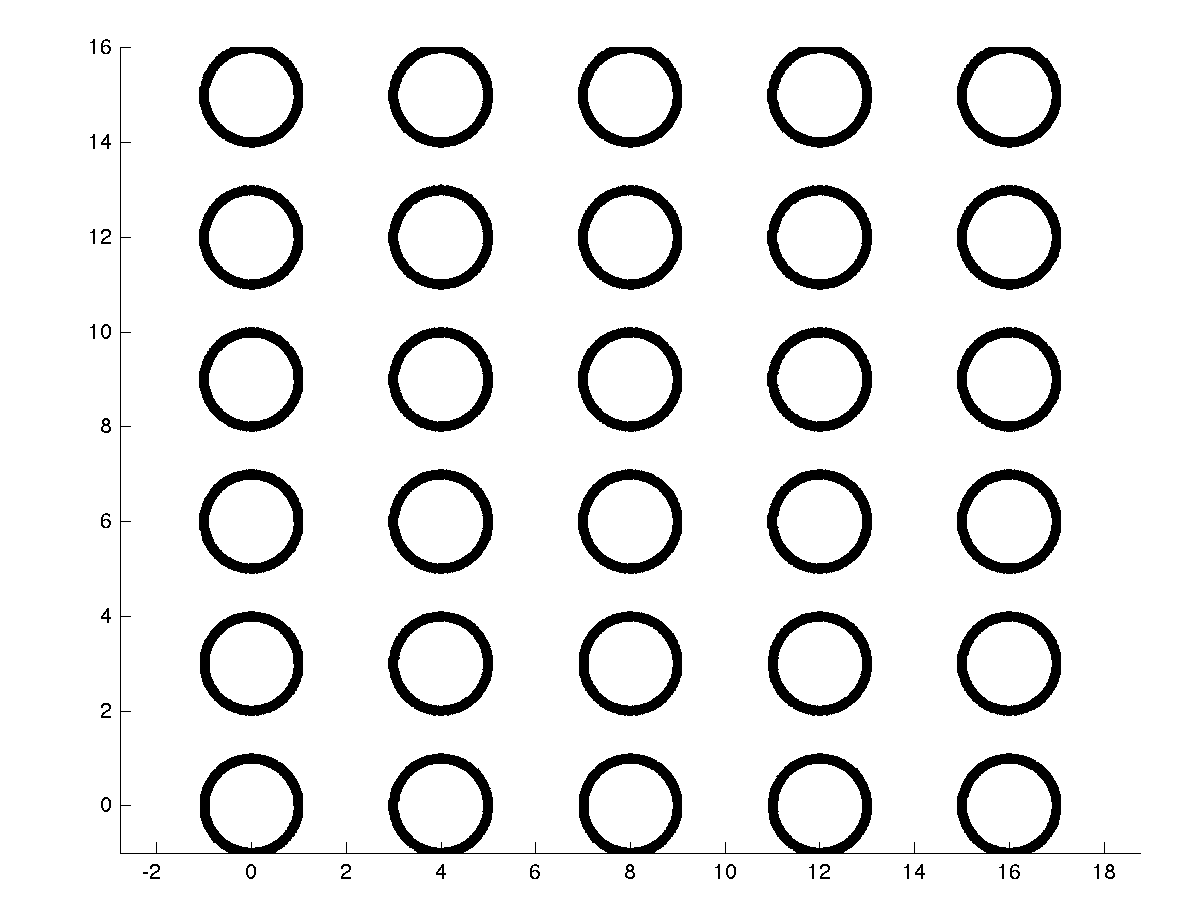
\includegraphics[width=0.45\textwidth]{./img/obstacles/rectangular.png}}
 \draw (10pt,-75pt) node[below]{\footnotesize $x_{1}$} ;
 \draw (-92pt,10pt) node[below]{\footnotesize $x_{2}$} ;
\end{tikzpicture}}\quad\subfigure[Triangular lattice]{\begin{tikzpicture}
 \pgftext{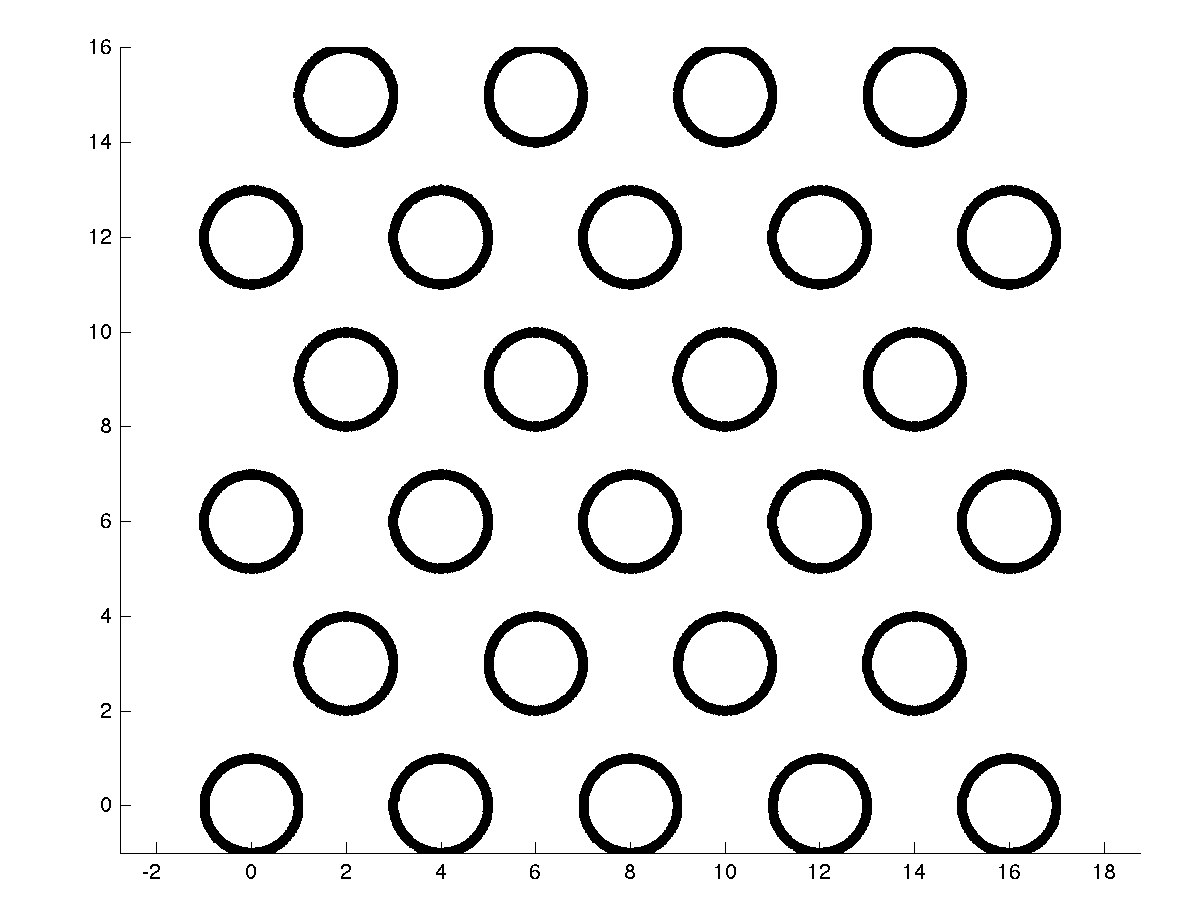
\includegraphics[width=0.45\textwidth]{./img/obstacles/triangular.png}}
 \draw (10pt,-75pt) node[below]{\footnotesize $x_{1}$} ;
 \draw (-92pt,10pt) node[below]{\footnotesize $x_{2}$} ;
\end{tikzpicture}}
\caption{Rectangular (left) and triangular (right) lattice with \code{bx}=3, \code{by}=4, \code{Nx} = 5, \code{Ny}=6.}
\label{fig:lattices}
\end{figure}


\subsubsection{Random placement}
\label{secFun:CreateRandomDisks}

\mudiff provides a function \CreateRandomDisks to randomly place \code{N\_scat} obstacles in a box $[\code{xmin}, \code{xmax}]\times[\code{ymin},\code{ymax}]$ with also a random radius. In its simplest version, the function is called as:
\begin{lstlisting}
[O, a] = CreateRandomDisks(xmin, xmax, ymin, ymax, N_scat);
\end{lstlisting}
In that case, \CreateRandomDisks builds \code{N\_scat} disk with unit radius in the desired box. The function takes care to not overlap the disks. Note that it is possible that the function does not succeed to place the obstacle (\eg if the user asks for too many obstacles in a small box) and hence a security has been set: only $500$ trials are allowed per disk. 

The function comes along with a large set of optional arguments:
\begin{lstlisting}
[O, a] = CreateRandomDisks(xmin, xmax, ymin, ymax, N_scat, 
           amin, amax, dmim, dmax, O_avoid, a_avoid, dmin_avoid, dmax_avoid);
\end{lstlisting}
where every additional arguments is optional (but the order must be kept (\code{amin} must be set, then \code{amax}, etc.!) and given by:
\begin{center}
\begin{tabular}{|c |c|c | p{10cm}|}
\hline Variable & Type & Default & Action\\\hline
\tabcode{amin} & scalar  & 1 & Minimal (random) radius of the obstacles allowed \\\hline
\tabcode{amax} & scalar  & 1 & Maximal (random) radius of the obstacles  allowed\\\hline
\tabcode{dmin} & scalar & \tabcode{realmin} & Minimal distance allowed between two obstacle (not between the centers!). Setting $\leq 0$  value will set \code{dmin} to \code{realmin} (\ie ignore it)\\\hline
\tabcode{dmax} & scalar & \tabcode{realmax} & Maximal distance allowed between two obstacle (not between the centers!). The maximal distance is quickly reached! Setting $\leq 0$  value will set \code{dmax} to \code{realmax} (\ie ignore it).\\\hline
\tabcode{O\_avoid} & $[2 \times N]$ & \tabcode{[]} & Center of \code{N} hole(s) where the obstacles must not overlap. Usefull for example for point source location.\\\hline
\tabcode{a\_avoid} & $[1 \times N]$ & \tabcode{[]} & Radii of the \code{N} holes\\\hline
\tabcode{dmin\_avoid} & $[1 \times N]$ & \tabcode{[]} & Minimal distance between an obstacle and a hole\\\hline
\end{tabular}
\end{center}
The ``holes'', represented by the \code{*\_avoid} arguments, are disks where the obstacles must not overlap, for example where a point source is emitting a wave. 

\paragraph{Example 1:} creating \code{N\_scat} random disks with random radii:
\begin{lstlisting}
[O, a] = CreateRandomDisks(xmin, xmax, ymin, ymax, N_scat, amin, amax);
\end{lstlisting}
\paragraph{Example 2:} building 7 obstacles in the box $[-10,10]\times[-10,10]$ with radii between $0.1$ and $0.5$. The disks must be separated at minimum by a distance of $0.1$ and without maximum value. The command is then:
\begin{lstlisting}
[O, a] = CreateRandomDisks(-10, 10, -10, 10, 7, 0.1, 0.5, 0.1, -1);
\end{lstlisting}
\paragraph{Example 3:} now imagine that a point source is located on $(2,2)$ and that the obstacles must be separated from the source from at least a distance of $0.3$, then the ``\code{*\_avoid}'' arguments can be used and command can be
\begin{lstlisting}
[O, a] = CreateRandomDisks(-10, 10, -10, 10, 7, 0.1, 0.5, 0.1, -1, [2;2], 0.3);
\end{lstlisting}
The disk centered on $(2,2)$ with radius $0.3$ will then be avoided. A second option is to set \code{a\_void} to zero and set the minimal distance \code{dmin\_avoid} to $0.3$:
\begin{lstlisting}
[O, a] = CreateRandomDisks(-10, 10, -10, 10, 7, 0.1, 0.5, 0.1, -1, [2;2], 0, 0.3);
\end{lstlisting}


\begin{remark}
\label{secFun:CheckPlacement}
To verify if a disk is well placed, \CreateRandomDisks calls \CheckPlacement function, which can also be useful for a user who is placing the obstacles manually.
\end{remark}

\subsubsection{Removing disks}
\label{secFun:RemoveDisk}

The function \RemoveDisk aims to remove some disks of the geometrical configuration, either disk by disk, by row or by column or by radius. This can be useful for example to delete a row of disks. Here is its syntax
\begin{lstlisting}
[O,a] = RemoveDisk(O_old, a_old, ...);
\end{lstlisting}
where \code{O\_old} and \code{a\_old} are the centers and radii of the current geometry. Without optional argument, the function has no effect. The available arguments are:
\begin{itemize}
\item \code{[O,a] = RemoveDisk(..., 'X', [X1, X2, .., XN]);}\\
Remove all the disks which center has its $x-$abscissa equal to \code{X1}, \code{X2}, \ldots, or \code{XN}
\item \code{[O,a] = RemoveDisk(...,  'Y', [Y1, Y2, ..., YN]);}\\
Remove all the disks which center has its $y$-ordinate \code{Y1}, \code{Y2}, \ldots, or \code{YN}
\item \code{[O,a] = RemoveDisk(..., 'XY', [[X1;Y1], [X2;Y2], ..., [XN;YN]]);}\\
Remove all the disks which center has for coordinates \code{[X1;Y1]}, \code{[X2;Y2]}, \ldots, or \code{[XN;YN]}
\item \code{[O,a] = RemoveDisk(..., 'Radius', [a1, a2, ..., aN]);}\\
Remove all the disk which radius is equal to \code{a1}, \code{a2}, \ldots, or \code{aN}
\item \code{[O,a] = RemoveDisk(..., 'Verbosity', VERBOSITY);}\\
set VERBOSITY to 0 to avoid display message, to 1 to only show results, and to $>1$ to see everything (default).
\item \code{[O,a] = RemoveDisk(..., 'Tol', TOL);}\\
Tolerance used for the conditional statement (default $10^{-10}$).
\end{itemize}

\paragraph{Example 1:} remove every obstacles that are either on the row of $x-$abscissa $1$ or on the column of $y-$ordinate $2.5$:
\begin{lstlisting}
[O,a] = RemoveDisk(O_old, a_old, 'X', 1, 'Y', 2.5);
\end{lstlisting}
\paragraph{Example 2:} remove the obstacles centered on $(2,5)$ and $(3,4)$:
\begin{lstlisting}
[O,a] = RemoveDisk(O_old, a_old, 'XY', [2, 3; 5, 4]);
\end{lstlisting}
\paragraph{Example 3:} create a periodic placement of $11$ by $11$ unit disks, separated by a distance of $1$ then remove the middle line and the middle column, as shown on figure \ref{fig:removeDisks}. The central disk is moreover centered on $(0,0)$.
\begin{lstlisting}
bx = 3; by = 3;
Nx = 11; Ny = 11;
O = RectangularLattice(bx, by, Nx, Ny, 'Center', [-15,-15]);
a = ones(1, size(O, 2));
[O, a] = RemoveDisk(O, a, 'X', 0, 'Y', 0);
\end{lstlisting}

\begin{figure}
\centering
\begin{tikzpicture}
 \pgftext{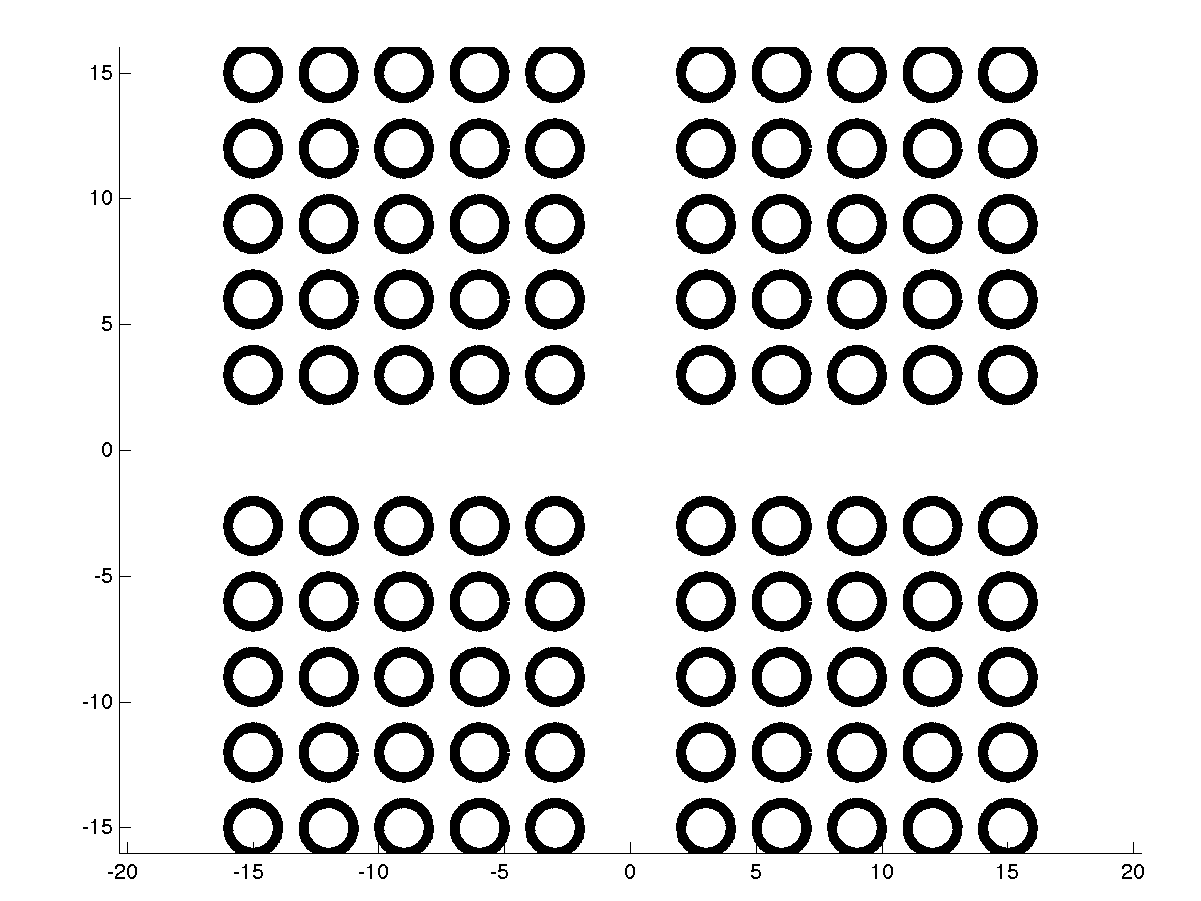
\includegraphics[width=0.45\textwidth]{./img/obstacles/removeDisks.png}}
 \draw (10pt,-75pt) node[below]{\footnotesize $x_{1}$} ;
 \draw (-92pt,10pt) node[below]{\footnotesize $x_{2}$} ;
\end{tikzpicture}
\caption{Periodic placement with a row and a column deleted.}
\label{fig:removeDisks}
\end{figure}



\subsection{Truncation of the Fourier series}
\label{secFun:FourierTruncation}

To help the user, the formula (\ref{eqEqInt:CFIEDapp}) has been computed in \mudiff. The values of $\Np$ are stored in a Matlab vector of size $[1\times\code{N\_scat}]$ called \code{M\_modes} in \mudiff. Computing \code{M\_modes} only involves the radii of the disks and the wavenumber \code{k}, which is assumed to be created by the user:
\begin{lstlisting}
M_modes = FourierTruncation(a, k);
\end{lstlisting}
The resulting vector is such that \code{M\_modes(p)}=$\Np$ where $\Np$ satisfies (\ref{eqEqInt:CFIEDapp}), with obviously a minimum value of $0$ (which consists of only one mode). If \code{k} is a vector (one wavenumber per obstacle), then \FourierTruncation compute formula (\ref{eqEqInt:CFIEDapp})  with \code{k(p)} as the wavenumber.

The following options are moreover availabe:
\begin{itemize}
\item \code{M\_modes = FourierTruncation(..., 'Min', MIN);}\\
To force a minimal value: \code{M\_modes(p)} is then either the min value between \code{MIN} and formula (\ref{eqEqInt:CFIEDapp}). 
\item\code{M\_modes = FourierTruncation(..., 'Tol', TOL);}
The tolerance, set by default to $10^{-10}$, is then set to \code{TOL}.
\end{itemize}

\subsection{Incident waves}

\subsubsection{Generalities}
\label{secFun:PlaneWave}
\label{secFun:DnPlaneWave}
\label{secFun:PointSource}
\label{secFun:DnPointSource}
\label{secFun:PlaneWavePrecond}
\label{secFun:DnPlaneWavePrecond}
\label{secFun:BlockPlaneWave}
\label{secFun:BlockDnPlaneWave}
\label{secFun:BlockPointSource}
\label{secFun:BlockDnPointSource}
\label{secFun:BlockPlaneWavePrecond}
\label{secFun:BlockDnPlaneWavePrecond}

Two different incident waves are available in the \mudiff toolbox: plane wave and point source wave. It should however be highlighted that the user can build his/her own incident wave. They are all located in \folder{PreProcessing/IncidentWave/}.

As explained in section \ref{secEqInt:SecondMembre}, a right-hand side $b$ is decomposed by blocks, each of these representing one obstacle: $b= (b_p)_{p=1,\ldots,\Nscat}$. A different condition can be applied on two different obstacles (\eg Dirichlet on $\Omega_1$ and Neumann on $\Omega_2$) or a different integral equation can be considered on it (\eg EFIE on $\Omega_1$ and MFIE on $\Omega_2$). To handle that, \mudiff builds each block separately thanks to \BlockIncidentWave, which computes the vector $b_p$. According to the input data, the function will build one of the available right-hand side described on table \ref{table:Uinc}.

On the other hand, the frontal function \IncidentWave computes the whole vector $b$. For every obstacle $p$, it calls \BlockIncidentWave and assembles the whole vector. 

In addition to this, for every incident waves, an interface function is available. They build the whole vector on only one pattern (trace of plane wave, normal derivative of point source wave, \ldots) but are very easy to use. They are located in the \folder{interface/} directory and their names are well chosen (see also table \ref{table:Uinc}, column \mudiff name): \PlaneWave, \PointSource, \DnPlaneWave,\ldots. Let us highlights that the help of the interface functions contains the mathematical description of the incident wave.

The two main functions, \BlockIncidentWave and \IncidentWave, are now detailed.

\subsubsection{\code{BlockIncidentWave}}
\label{secFun:BlockIncidentWave}

This functions computes the block vector of \textbf{the opposite of} the coefficients of an incident wave, either the trace of the normal derivative trace, on one of the obstacles, in the Fourier bases. Its syntax is
\begin{lstlisting}
Bp = BlockIncidentWave(Op, ap, Np, k, TypeOfWave, Param);
\end{lstlisting}
where \code{TypeOfWave} is a scalar value specifying the incident wave (see table \ref{table:Uinc}) and \code{Param} is the parameter of the wave: angle of direction, position of a point source, \ldots. The returned value \code{Bp} is a column vector of length $2\code{Np}+1$.
\begin{table}
\begin{tabular}{|c| c |c| p{9cm}| }
\hline Value & \mudiff name & Param & Type\\\hline
1 & \code{PlaneWave} & \code{beta\_inc} & Trace of a plane wave of angle of direction \code{beta\_inc}. A plane wave is defined by $e^{ik(\cos(\beta)x + \sin(\beta)y}$.\\\hline
2 & \code{DnPlaneWave} & \code{beta\_inc} & Normal derivative of a plane wave of angle of direction \code{beta\_inc}.\\\hline
3 & \code{PointSource} & \code{XS} & Trace of the wave emitted by a point source placed on \code{XS}. Such a wave is defined in \mudiff by $i/4\Hz(k\|\xx-\xx_s\|)$.\\\hline
4 & \code{DnPointSource} & \code{XS} & Normal derivative of the trace of the wave emitted by a point source placed on \code{XS}.\\\hline
5 & \code{PlaneWavePrecond} & \code{beta\_inc} & Same as \code{PlaneWave} but multiplied by the inverse diagonal of the single-layer diagonal block operator (see section \ref{} on single scattering preconditioner). \\\hline
6 & \code{DnPlaneWavePrecond} & \code{beta\_inc} & Same as \code{DnPlaneWave} but multiplied by the inverse diagonal of the double-layer diagonal block operator. \\\hline
\end{tabular}
\caption{Available right-hand sides}
\label{table:Uinc}
\end{table}

\subsubsection{\code{IncidentWave}}
\label{secFun:IncidentWave}

\begin{lstlisting}
B = IncidentWave(O, a, M_modes, k, TypeOfWave, Param)
\end{lstlisting}
The resulting vector \code{B} is of size $\sum_{p=1}^{\Nscat}(2\code{M\_modes}(p)+1)$. The value \code{Param} is the same as for \BlockIncidentWave whereas \code{TypeOfWave} is a vector of size $\Nscat$ where \code{TypeOfWave}(p) is the desired choice for the block $b_p$. In other word, the block $b_p$ will be built by calling \code{BlockIncidentWave(Op, ap, Np, k, TypeOfWave, Param);}. To simplify, if \code{TypeOfWave} is a scalar value, then it is considered as a vector of the same scalar value.

\paragraph{Example1:} building a vector associated to the trace of an incident plane wave of direction \code{beta\_inc} is done thanks to the following command (the ``$1$ argument'' refers to \code{PlaneWave}):
\begin{lstlisting}
B = IncidentWave(O, a, M_modes, k,  1, beta_inc);
\end{lstlisting}
or using the interface function
\begin{lstlisting}
B = PlaneWave(O, a, M_modes, k, beta_inc);
\end{lstlisting}
\paragraph{Example 2:} For two obstacles and a point source centered on $(1,2)$, if $b_1$ is the trace of the wave and $b_2$ is the normal derivative trace, then
\begin{lstlisting}
B = IncidentWave(O, a, M_modes, k,  [3;4],[1;2]);
\end{lstlisting}
In other words, this builds the vector (\code{[3,4]} can be translated as \code{PointSource, DnPointSource}):
$$
b = \left(\begin{array}{c}
-\uinc|_{\Gamma_1}\\
-\dn\uinc|_{\Gamma_2}\\
\end{array}\right),
$$
where $\uinc = \frac{i}{4}\Hz(k\|\xx-\xx_s\|)$, with $\xx_s = [1,2]$.
\begin{remark}
Remember that the resulting vector corresponds to the opposite of the trace or normal derivative trace!
\end{remark}


\section{Integral operators}
\label{sec:ResolutionMuDiff}

\subsection{Generalities}

The functions defining the integral operators are in the directory \folder{IntOperators/} which has the \folder{Dense/}
and \folder{Sparse/} subdirectories for the dense (matrix) and sparse (@function) representations of the four basic integral operators used in scattering,
\ie $\Lb$, $\Mb$, $\Nb$ and $\Db$, given in their infinite version by respectively (\ref{eq:InfL}), (\ref{eq:InfM}), (\ref{eq:InfN}) and (\ref{eq:InfD}). Preconditioned versions of the operators by their single scattering operators \cite{Thi14}. In fact and following Proposition \ref{prop:SingleScat}, only $\widehat{L}L$ (EFIE Dirichlet) and $\widehat{D}D$ (EFIE Neumann) are available, as they are the only one needed for the Dirichlet and Neumann problems. These operators have moreover an analytic expression of every of their coefficients (see equations (\ref{eq:LL}) and (\ref{eq:DD}), in the infinite matrices case).

Two different type of storage are available with the \mudiff toolbox: dense and sparse. The assembly of matrix is however similar for both cases (only a few differences). \mudiff is close to the mathematics for the assembly process, in the sense that the matrix $\Ab$ of an integral operator is built block by block ($\Abpq$). For both storage, two main functions exist: a ``block'' function (\BlockIntegralOperator and \SpBlockIntegralOperator) and a whole matrix function (\IntegralOperator and \SpIntegralOperator), which assembles every blocks into one matrix. This separation permits to the user to either build a ``simple'' matrix of one operator or to construct a more ``complex'' matrix where each block represents a different operator or a linear combination of them. Note also that, every operator has functions of interface (located in \folder{Dense/Interface} or \folder{Sparse/Interface} folders). For example \SingleLayer is the interface function of \IntegralOperator to build the single-layer operator, and \BlockSingleLayer the one of \BlockIntegralOperator. The same applies for the sparse storage with a prefix \code{Sp}:  \SpSingleLayer,  \SpBlockSingleLayer.


The dense storage should be preferred for solving small scale problem, when the memory and the CPU cost is not a problem, where the sparse storage must be used when the limits are reached. For the sparse storage, which is detailed later, the matrices are stored as vectors and the matrix-vector product is then fast. The drawback being however some instability, in particular when the truncation of the Fourier series is not done properly. The formula (\ref{eqEqInt:CFIEDapp}) seems to give a stable result though \cite{AntChnRam08}.



%Two different type of storage are provided with the \mudiff toolbox: dense and sparse. The dense storage the whole matrix in memory whereas the sparse version uses the special structure of the matrix of an integral operator to store it. The sparse storage in \mudiff and this user guide has nothing to deal with the sparse storage provided in \matlab such as \texttt{sparse} function. The dense storage is easier to use and works pretty well for small scale problems. It also presents the advantage of providing the whole matrix of the integral operator, which can be useful for spectrum analysis for example. On the other hand, for a large number of circular obstacles and/or for large frequency, the memory storage becomes too important and the sparse version must be used. One should be however careful: the sparse matrix-vector product, based on the cross-correlation (\texttt{xcorr} \matlab function), is very sensitive to the number of modes chosen in the truncation of the Fourier series. Indeed, if too many modes are kept, the matrix-vector product show to be unstable. The formula (\ref{eqEqInt:CFIEDapp}) seems to provide stability.
%
%To explain how the code works, let us take an example of one of the four boundary integral operator $L,M,N$ or $D$ being discretized as a generic matrix $\Ab = (\Abpq)_{1\leq p,q\leq \Nscat}$. Let us highlight that \mudiff can manage more complexe matrices, where two different blocks are not the discretization of the same operators or can even be a linear combination of operators. Nevertheless, if $\Ap$ is one of the four boundary integral operators, then as highlighted in previous chapter, $\Ab$ has the following structure, for $p,q=1,\ldots,\Nscat$ and $p\neq q$:
%\begin{itemize}
%\item $\Abpp$ is diagonal.
%\item $\Abpq$ is full and can be divided as $\Abpq = \AbpqL\Tbpq\AbpqR$ where $\AbpqL$ and $\AbpqR$ are diagonal and called respectively the left and right part, and $\Tbpq = (\Tbpqmn))$, with $\Tbpqmn = i\pi e^{??}H_0^{(1)}(k\bpq)$, is a Toeplitz matrix.
%\end{itemize}
%In the sparse version, diagonal submatrices $\Abpp,\AbpqL$ and $\AbpqR$  are stored as a vector of size respectively $2\Np+1$, $2\Np+1$ and $2\Nq+1$, and the Toeplitz matrices $\Tbpq$ are stored as vectors of size $2\Np+2\Nq-1$.
%
%This section is naturally divided in two part, the first being devoted to the dense storage and the second to the sparse version. The assembly, the storage and the usage of the matrices being significantly different.

\subsection{Available integral operators and numbering}
\label{seccode:IntOp}
\label{secFun:BlockSingleLayer}
\label{secFun:BlockDnSingleLayer}
\label{secFun:BlockDoubleLayer}
\label{secFun:BlockDnDoubleLayer}
\label{secFun:BlockPrecondDirichlet}
\label{secFun:BlockPrecondNeumann}
\label{secFun:BlockCalderonProjector}
\label{secFun:BlockIdentity}
\label{secFun:SingleLayer}
\label{secFun:DnSingleLayer}
\label{secFun:DoubleLayer}
\label{secFun:DnDoubleLayer}
\label{secFun:PrecondDirichlet}
\label{secFun:PrecondNeumann}
\label{secFun:CalderonProjector}
\label{secFun:Identity}

As for the incident wave, for every operator, there exists a function that build the whole operator for the multiple scattering problem, both for dense and sparse storage. The available operators are listed on table \ref{table:IntOp}, with their unique identifier (integer), their name in \mudiff (useful to get their interface functions) and their definition.

\begin{table}
\begin{center}\begin{tabular}{|c| c| c|c|}
\hline Int. Op. & Identifier & Function & Definition for $\xx\in\Gamma$\\\hline\hline
- & 0 & - & Zero operator (null matrix)\\\hline
$I$ & 1 & \tabcode{Identity} & Identity\\\hline
$L$ & 2 & \tabcode{SingleLayer} & $\dsp L\rho(\xx) = \int_{\Gamma} G(\xx,\yy) \rho(\yy)\dd\yy$\\[0.25cm]\hline
$M$ & 3 & \tabcode{DoubleLayer} & $\dsp M\lambda(\xx) = -\int_{\Gamma} \dny G(\xx,\yy) \lambda(\yy)\dd\yy$\\[0.25cm]\hline
$N$ & 4 & \tabcode{DnSingleLayer} & $\dsp N\rho(\xx) = \dnx\int_{\Gamma} G(\xx,\yy) \rho(\yy)\dd\yy$\\[0.25cm]\hline
$D$ & 5 & \tabcode{DnDoubleLayer} & $\dsp D\lambda(\xx) = -\dnx\int_{\Gamma} \dny G(\xx,\yy) \lambda(\yy)\dd\yy$\\[0.25cm]\hline
$\hat{L}L$ & 6 & \tabcode{PrecondDirichlet} & Single-Layer preconditioned by its diagonal\\[0.25cm]\hline
$\hat{D}D$& 7 & \tabcode{PrecondNeumann} & Dn Double-Layer preconditioned by its diagonal\\[0.25cm]\hline
\end{tabular}\end{center}
\caption{Available operators, their unique identifier, function name (interface) and the mathematical definition. The zero function does not have an interface function and the sparse version is obtained by prefixing by \code{Sp} (\SpSingleLayer, \SpDnDoubleLayer,\ldots). The block interface functions are also prefixed by ``\code{Block}'' (\SpBlockSingleLayer, \BlockSingleLayer,\ldots)}
\label{table:IntOp}
\end{table}


\subsection{Dense storage}
\subsubsection{Building a block $\Abpq$}
\label{secFun:BlockIntegralOperator}

A sub matrix block can be created with the function \BlockIntegralOperator:
\begin{lstlisting}
Apq = BlockIntegralOperator(Op, ap, Np, Oq, aq, Nq, k, TypeOfOperator, Weight);
\end{lstlisting}
The \code{Weight} argument is optional and set to $1$ by default. The quantity \code{TypeOfOperator} specifies the integral operator to compute, thanks to the numbering of Table \ref{table:IntOp}. If \code{TypeOfOperator} is a scalar (\eg $=2$) then the resulting matrix \code{Apq} is the submatrix of the associated operator (\eg $\Lbpq$). If \code{TypeOfOperator} is a row (\eg \code{[1,3]}) then the sum of the two operators is done (\eg $\Ibpq+\Mbpq$). Finally the \code{Weight} quantity, of the same size as \code{TypeOfOperator}, is the constant to multiply the block with. The block is hence:
$$
\Abpq = \sum_{\ell=1}^{N}\code{Weight}(\ell).\code{Operator}(\ell)
$$
where \code{Operator}$(\ell)$ is one of the integral operator.

\paragraph{Example 1:} Building the single-layer block $\Lbpq$:
\begin{lstlisting}
Apq = BlockIntegralOperator(Op, ap, Np, Oq, aq, Nq, k, 1);
\end{lstlisting}
\paragraph{Example 2:} Build the whole matrix $0.5\Ibpq + \Nbpq$, appearing in the MFIE (\ref{eq:MFIE}):
\begin{lstlisting}
Apq = BlockIntegralOperator(Op, ap, Np, Oq, aq, Nq, k, [1, 4], [0.5, 1]);
\end{lstlisting}
\paragraph{Example 3:} The sum of the four blocks: $0.5\Lbpq + 1.5\Mbpq + 2.5\Nbpq + 3.5\Dbpq$:
\begin{lstlisting}
Apq = BlockIntegralOperator(Op, ap, Np, Oq, aq, Nq, k, [2, 3, 4, 5], 
                         [0.5, 1.5, 2.5, 3.5]);
\end{lstlisting}


\subsubsection{Assemble the matrix $\Ab$}
\label{secFun:IntegralOperator}

Now that the construction of a block is well understood, building a matrix is very easy thanks to the frontal function
\begin{lstlisting}
A = IntegralOperator(O, a, M_modes, k, TypeOfOperator, Weight);
\end{lstlisting}
As for \BlockIntegralOperator, the quantity \code{Weight} is optional and set to $1$ by default. Roughly speaking, \IntegralOperator will loop on every obstacle $p$ and $q$ and launch the following command
\begin{lstlisting}
Apq = BlockIntegralOperator(O(:,p), a(p), M_modes(p), O(:,q), a(q), M_modes(q), 
                                                    k, Tpq, Wpq);
\end{lstlisting}
and places \code{Apq} in the right block of the whole matrix. The quantities \code{Tpq} and \code{Wpq} are given by \code{TypeOfOperator} and \code{Weight} such that (\code{Weight} is of the same size of \code{TypeOfOperator} and so \code{Wpq} follows the same rules as \code{Tpq}):
\begin{itemize}
\item If \code{TypeOfOperator} is a scalar then \code{Tpq} = \code{TypeOfOperator}. 
\item If \code{TypeOfOperator} is a row or a column vector then \code{Tpq} is an array given by \code{Tpq} = \code{TypeOfOperator}. 
\item If \code{TypeOfOperator} is a matrix then \code{Tpq} = \code{TypeOfOperator(p,q)}. 
\item If \code{TypeOfOperator} is a $3D-$array then \code{Tpq} is an array and is given by \code{Tpq(:)} = \code{TypeOfOperator(p,q,:)}. 
\end{itemize}
%
%For example, this matrix will give,
%$$
%\left(\begin{array}{c c}
%2& 3\\
%4&5
%\end{array}\right)
%\longrightarrow
%\left(\begin{array}{c c}
%L^{1,1}& M^{2,1}\\
%N^{1,2} & D^{2,2}
%\end{array}\right)
%$$


\paragraph{Example 1:} The single-layer potential $L$
\begin{lstlisting}
L = IntegralOperator(O, a, M_modes, k, 2);
\end{lstlisting}
\paragraph{Example 2:} The operator of the MFIE for a Dirichlet boundary condition (\ref{eq:MFIE}), $0.5I + N$:
\begin{lstlisting}
A_MFIE = IntegralOperator(O, a, M_modes, k, [1,4], [0.5,1]);
\end{lstlisting}
\paragraph{Example 3:} The following operator for two obstacles only
$$
\left(\begin{array}{c c}
0.5 I_{1,1}+ M_{1,1} & L_{1,2}\\
D_{2,1} & 0.5 I_{2,2}+N_{2,2}
\end{array}\right)
$$
can be computed using a $3D$ array and the null operator:
\begin{lstlisting}
TypeOfOp = zeros(2,2,2); Weight = zeros(2,2,2);
TypeOfOp(:, 1,1) = [1, 3]; Weight(:, 1,1) = [0.5, 1]; %block A_{1,1}
TypeOfOp(:, 1,2) = [2, 0]; Weight(:, 1,2) = [1, 0]; %block A_{1,2}
TypeOfOp(:, 2,1) = [5, 0]; Weight(:, 2,1) = [1, 0]; %block A_{2,1}
TypeOfOp(:, 2,2) = [1, 4]; Weight(:, 2,2) = [0.5, 1]; %block A_{2,2}
A = IntegralOperator(O, a, M_modes, k, TypeOfOp, Weight);
\end{lstlisting}
\paragraph{Example 4:} The Brakhage-Werner integral equation for a Dirichlet problem (\ref{eqEqInt:BW})
\begin{lstlisting}
k = 1;
beta_inc = pi;
eta = i/k;
Uinc = PlaneWave(O, a, M_modes, k, beta_inc);
A = IntegralOperator(O, a, M_modes, k, [1, 2, 3], [0.5, -eta_BW, -1]);
psi = A \ Uinc;
\end{lstlisting}

\subsection{Sparse storage}
\label{secFun:SpBlockSingleLayer}
\label{secFun:SpBlockDnSingleLayer}
\label{secFun:SpBlockDoubleLayer}
\label{secFun:SpBlockDnDoubleLayer}
\label{secFun:SpBlockPrecondDirichlet}
\label{secFun:SpBlockPrecondNeumann}
\label{secFun:SpSingleLayer}
\label{secFun:SpDnSingleLayer}
\label{secFun:SpDoubleLayer}
\label{secFun:SpDnDoubleLayer}
\label{secFun:SpPrecondDirichlet}
\label{secFun:SpPrecondNeumann}
\label{secFun:SpIdentity}

Storing the matrices in a sparse way leads to a significant reduction in memory storage and a faster matrix-vector product. The linear system must then however be solved using an iterative solver only, as the matrix is no more fully stored. Combining linearly the matrices is still possible but this is done during the matrix-vector product. Indeed, summing two matrices of two different integral operators is not guaranteed to keep the special structure. If the problem involves (at least) two different integral operators, they must hence be computed separately.

\subsubsection{Compact storage}

To explain how the matrix is stored using \mudiff sparse storage, let $\Ab$ be the matrix of one of the four integral operators $L,M,N$ or $D$. The matrix $\Ab$ has the following special structure (for $p,q=1,\ldots,M$ and $p\neq q$):
\begin{itemize}
\item $\Abpp$ is diagonal
\item $\Abpq$ is full and can be divided as $\Abpq = \AbpqL\Tbpq\AbpqR$ where $\AbpqL$ and $\AbpqR$ are diagonal and called respectively the left and right part, and $\Tbpq = (\Tbpqmn))$, with $\Tbpqmn = i\pi e^{i(n-m)\alpha_{pq}}H_{n-m}^{(1)}(k\bpq)$, is a Toeplitz matrix: $\Tbpqmn = \Tbpq_{m+1,n+1}$.
\end{itemize}

The idea is that the diagonal matrices can be stored as a vector containing the diagonal only. A matrix-vector product between a diagonal matrix and a vector is then simply a point-to-point multiplication. The Toeplitz matrix can also be stored in a compact form as a vector and the matrix-vector product is handled by a cross-correlation (based on FFT). 

The diagonals part are stored in the $3D$ arrays $\AbL$ and $\AbR$ (``L'' for left part and ``R'' for the right part). The left part, $\AbL$ also carries the diagonal part of the matrix:
$$
\AbL(:,p,q) = \begin{cases}
\diag(\Abpp) & \text{ if }p=q,\\
\diag(\AbpqL) & \text{ otherwise,}
\end{cases}\qquad
\AbR(:,p,q) = \begin{cases}
0 & \text{ if }p=q,\\
\diag(\AbpqR) & \text{ otherwise.}
\end{cases}
$$
The matrix $\Tbpq$, of size $(2\Np+1) \times (2\Nq+1)$ is then also compacted as a Toeplitz matrix has the following structure
$$
\Tbpq = \left(\begin{array}{c c c c c}
t_1 & t_2 & t_3 & \ldots & t_{(2\Nq+1)} \\
t_{(2\Nq+1)+1} & t_{1} & t_{2} & \ldots & t_{(2\Nq+1)-1}\\
t_{(2\Nq+1)+2} & t_{(2\Nq+1)+1} & t_{1} & \ldots & t_{(2\Nq+1)-2}\\
\vdots & \ddots & \ddots& \ddots& \vdots\\
%t_{(2\Nq+1)+(2\Np+1)-2} & t_{(2\Nq+1)+(2\Np+1)-3} & t_{(2\Nq+1)+(2\Np+1)-4} &   \ldots & t_{(2\Np+1)+1}\\
t_{(2\Nq+1)+(2\Np+1)-1} & t_{(2\Nq+1)+(2\Np+1)-2} & t_{(2\Nq+1)+(2\Np+1)-3} &   \ldots  & t_{(2\Nq+1)-(2\Np+1)+1}
\end{array}\right)
$$
Clearly, the root vector containing the first row and the first column is enough to rebuild the matrix. This root vector, called $\AbpqM$, is of size $(2\Np+1)+ (2\Nq+1)-1 = 2\Np +2\Nq+1$ and such that:
$$
\AbpqM = \left(\begin{array}{c}
t_{(2\Nq+1)+(2\Np+1)-1}\\
t_{(2\Nq+1)+(2\Np+1)-2}\\
\vdots\\
t_{(2\Nq+1)+2}\\
t_{(2\Nq+1)+1}\\
t_{1}\\
t_{2}\\
t_{3} \\
\vdots\\
t_{(2\Nq+1), 1}\\
\end{array}\right).
$$
Finally, all these root vectors are stored in the $3D$ array $\AbM$:
$$
\AbM(:,p,q) = \begin{cases}
0 & \text{ if }p=q,\\
\AbpqM & \text{ otherwise.}
\end{cases}
$$

The whole matrix $\Ab$ is thus stored in three different parts: $\AbL$, $\AbM$ and $\AbR$. From the computer point of view, as a $3D$ array has a fix size in each direction, the second and third dimension of the arrays are both of size \code{N\_scat} and the length in the first dimension is given by:
\begin{center}
\begin{tabular}{| l | l | l | l |}
\hline $3D$-array & \multicolumn{3}{c|}{Length in the dimension\ldots}\\\cline{2-4}
& $1$ & $2$ & $3$\\\hline
$\AbL$ & $\dsp \max_p(2\Np+1)$ & \tabcode{N\_scat}& \tabcode{N\_scat}\\[0.2cm]\hline
$\AbM$ & $\dsp \max_{p}\max_{q\neq p}\left[(2\Np+1)+(2\Nq+1)-1\right]$& \tabcode{N\_scat}& \tabcode{N\_scat}\\[0.2cm]\hline
$\AbR$ & $\dsp \max_p(2\Np+1)$& \tabcode{N\_scat}& \tabcode{N\_scat}\\[0.2cm]\hline
\end{tabular}\end{center}
With this constraint, the vector $\AbL(:,p,q)$ can be larger than $2\Np+1$ and thus $\AbpqL$ must be extracted: $\AbpqL = \AbL(1:2\Np+1, p, p)$. The same occurs for $\AbM$ and $\AbR$. 

Finally, these $3D$ arrays are merged into a cell \code{A}, representing the matrix $\Ab$, such that, using the Matlab notations:
$$
\code{A}\{1\} = \AbL,\qquad \code{A}\{2\} = \AbM,\qquad\code{A}\{3\} = \AbR.
$$

\subsubsection{Fast matrix-vector product}

The matrix vector product between $\Ab$ and a vector $X$ is divided in different smaller operations. Let us look at $Y=\Ab X$ and more particularly at the $p^{th}$ component
$$
Y_p = \sum_{q} \Abpq X_q.
$$
Using the previous notations, it can be rewritten as
$$
Y_p = \AbppL X_p + \sum_{q\neq p} \AbpqL (\AbpqM (\AbpqR X_q)).
$$
As $\AbppL$, $\AbpqL$ and $\AbpqR$ are all diagonal (and stored as a vector), these matrix-vector products are easy to compute. The only difficulty is located in $\AbpqM Z_q$ (where $Z_q=\AbpqR X_q$), but it can be achieved in a fast way. Indeed, the discrete cross correlation product (\code{xcorr}) between $\AbpqM$ and $Z_q$ gives
$$
\widetilde{W}_q = \code{xcorr}(Z_q, \overline{\AbpqM}),
$$
where the over bar denotes a complex conjugation. And the result $W_q$ is then extracted from $\widetilde{W}_q$ by
$$
W_q = \widetilde{W}_q(2\Nq+1:2\Nq+1+2\Np).
$$
The matrix vector product between $\Ab$ and $X$ is then done in a fast way (cross correlation is fast using Fourier).


\subsubsection{\mudiff: assemble the matrix}
\label{secFun:SpBlockIntegralOperator}
\label{secFun:SpIntegralOperator}

The assembly process is very similar to the dense one, the difference being the prefix \code{Sp}. The block function is then called by
\begin{lstlisting}
SpBlockIntegralOperator(Op, ap, Np, Oq, aq, Nq, Nmax, k, TypeOfOperator, Weight);
\end{lstlisting}
The function returns three vectors corresponding to $\AbpqL$, $\AbpqM$ and $\AbpqR$. The major difference here is that \textbf{no linear combination of operators can be done during the assembly process} for the sparse representation. The quantity \code{TypeOfOperator} cannot hence be a vector but only a scalar. On the other hand, the full assembly of a matrix can be done through
\begin{lstlisting}
A = SpIntegralOperator(O, a, M_modes, k, TypeOfOperator, Weight);
\end{lstlisting}
The result is a Matlab \code{cell} of three component, where each of them is a $3D-$array. The quantity \code{TypeOfOperator} can be a scalar or a matrix (not a $3D$ array nor a vector!). If \code{TypeOfOperator} is a matrix, then the block $\Abpq$ is assumed to be of type \code{TypeOfOperator(p,q)}. The linear combination of operators can still be done, but must be specified in the matrix-vector product (see below). Note that a function exists to add the (weighted-)identity to a sparse operator (see below).

\paragraph{Example 1:} Creation of \mudiff sparse matrix of the single-layer operator $L$
\begin{lstlisting}
L = SpIntegralOperator(O, a, M_modes, k, 2);
\end{lstlisting}
\code{L} is now a cell of $3$ components! Note that we can use the interface function
\begin{lstlisting}
L = SpSingleLayer(O, a, M_modes, k);
\end{lstlisting}
\paragraph{Example 2:} For two obstacles, building the following matrix 
$$
\left(\begin{array}{c c}
M_{1,1} & 0.5L_{1,2}\\
1.5D_{2,1} & 2.5N_{2,2}
\end{array}\right)
$$
can be done with the below commands
\begin{lstlisting}
TypeOfOp = zeros(2,2); Weight = zeros(2,2);
TypeOfOp(1,1) = [3]; Weight(1,1) = [1]; %block A_{1,1}
TypeOfOp(1,2) = [2,]; Weight(1,2) = [0.5]; %block A_{1,2}
TypeOfOp(2,1) = [5]; Weight(2,1) = [1.5]; %block A_{2,1}
TypeOfOp(2,2) = [4]; Weight(2,2) = [2.5]; %block A_{2,2}
A = SpIntegralOperator(O, a, M_modes, k, TypeOfOp, Weight);
\end{lstlisting}

\subsubsection{Assembly: adding the identity}
\label{secFun:SpAssIdentity}

It is possible to add the identity (multiplied by a constant) to a sparse operator:
\begin{lstlisting}
A = SpAddIdentity(A, alpha, M_modes);
\end{lstlisting}
which simply returns $A = A+\alpha I$.

\paragraph{Example 1:} If \code{L} is the sparse representation of the single-layer operator, then
\begin{lstlisting}
L = SpIntegralOperator(O, a, M_modes, k, 2);
alpha_L = SpAddIdentity(L, 0.5, M_modes);
\end{lstlisting}
will compute $0.5L$.

\subsubsection{\mudiff: sparse matrix-vector product}
\label{secFun:SpMatVec}
\label{secFun:SpSingleMatVec}

A matrix vector product $Y = \Ab X$ is done thanks to 
\begin{lstlisting}
Y = SpMatVec(X, M_modes, ListOfOperators, Weight);
\end{lstlisting}
where \code{Weight} is optional. \code{ListOfOperators} is a \textbf{Matlab cell} (not an array! Make use of $\{\cdot\}$ instead of $[\cdot]$) containing every sparse matrices that the user want to use. The linear combination of the operators is done at that time at each matrix-vector product.

\paragraph{Example 1:} Computing $Y = \Lb X$ is done as follows:
\begin{lstlisting}
SpL = SpIntegralOperator(O, a, M_modes, k, 2);
Y = SpMatVec(X, M_modes, SpL);
\end{lstlisting}
\paragraph{Example 2:} Calculating $Y =(0.5*I + N)X$, where $I$ is the identity (\textbf{Beware the $\{\cdot\}$ !}):
\begin{lstlisting}
SpI = SpIdentity(O, a, M_modes);
SpN = SpDnSingleLayer(O, a, M_modes, k);
Y = SpMatVec(X, M_modes, {SpI, SpN}, [0.5, 1]);
\end{lstlisting}
This could also be done using \SpAddIdentity function:
\begin{lstlisting}
SpN = SpDnSingleLayer(O, a, M_modes, k);
A = SpAddIdentity(SpN, 0.5, M_modes);
Y = SpMatVec(X, M_modes, A);
\end{lstlisting}

\subsubsection{Solving a linear system}

Now that the matrices and the right hand side have been assembled, the sparse linear system can solved iteratively. Using for example the GMRES solver \cite{SaaSch86}, the syntax to solve\ldots
\paragraph{Example 1: The EFIE (\ref{eq:EFIE}):} $L\rho = -\uinc|_{\Gamma}$, would be
\begin{lstlisting}
SpL = SpSingleLayer(O, a, M_modes, k);
Uinc = PlaneWave(O, a, M_modes, k, beta_inc);
rho = gmres(@(X)SpMatVec(X, M_modes, SpL), Uinc);
\end{lstlisting}
\paragraph{Example 2: The MFIE (\ref{eq:MFIE}):} $(I/2+N)\rho = -\dn\uinc|_{\Gamma}$:
\begin{lstlisting}
SpN = SpDnSingleLayer(O, a, M_modes, k);
SpI = SpIdentity(O, a, M_modes);
DnUinc = DnPlaneWave(O, a, M_modes, k, beta_inc);
rho = gmres(@(X)SpMatVec(X, M_modes, {SpI, SpN}, [0.5, 1]), DnUinc);
\end{lstlisting}
or using the \SpAddIdentity function
\begin{lstlisting}
SpAMFIE = SpDnSingleLayer(O, a, M_modes, k);
SpAMFIE = SpAddIdentity(SpAMFIE, 0.5, M_modes);
DnUinc = DnPlaneWave(O, a, M_modes, k, beta_inc);
rho = gmres(@(X)SpMatVec(X, M_modes, SpAMFIE), DnUinc);
\end{lstlisting}
\paragraph{Example 3: The Brakhage-Werner integral equation} for a Dirichlet problem (\ref{eqEqInt:BW})
\begin{lstlisting}
k = 1;
beta_inc = pi;
eta = i/k;
Uinc = PlaneWave(O, a, M_modes, k, beta_inc);
SpA = SpIntegralOperator(O, a, M_modes, k, [1, 2, 3], [0.5, -eta_BW, -1]);
psi = gmres(@(X)SpMatVec(X, M_modes, SpA), Uinc);
\end{lstlisting}


\section{Post-Processing}
\label{sec:PostProcessing}

Now that the system has been solved, the next step is to display some results. The \mudiff toolbox proposes some post-processing features such as computing the far-field (fast) or the near-field of the wave on a grid (Matlab \code{meshgrid}) or on some points only. In addition, other features are available such as drawing the disks on figures or the incident field. Both the near- and far-field computations can be done for a linear combination of a single- and double-layer potentials $\Lop\rho + \Mop\lambda$, only one of them (\eg $\Lop\rho$) or with the same density $(\Lop+\Mop)\psi$, with a single command line. Every post-processing functions are located in the \folder{PostProcessing/} directory.

\subsubsection{Far field}
\label{secFun:FarField}
\label{secFun:FarFieldSingleLayer}
\label{secFun:FarFieldDoublleLayer}

The far field of the single- and double-layer potentials
$$
\sum_{p=1}^{\Nscat}\eta_p\Lop_p\rho_p + \gamma_p\Mop_p\lambda_p,
$$
is given by equation (\ref{eq:FFFourier}). The \FarField function does the job properly:
\begin{lstlisting}
F = FarField(O, a, M_modes, k, theta, Density, Weight);
\end{lstlisting}
where the parameters are:
\begin{itemize}
\item \code{theta} is the vector of receiving angles (in rad.)
\item \code{Density} is either $\rho$, $\lambda$ or both. If \code{Density} is a column vector then \code{Density(:,2)} = \code{Density(:,1)} and only one density is used both for the single- and the double-layer potentials contribution. If \code{Density} has $2$ columns, then \code{Density(:,1)} is considered to be the single-layer density and \code{Density(:,2)} the double-layer density.
\item \code{Weight} is the weights to apply to the $\Nscat$ volumic integral operators ($\eta_p$ and $\gamma_p$). The quantity \code{Weight} is of size either $[1\times2]$ or $[1\times\Nscat]$. The first column of \code{Weight} is applied to the single-layer potentials and the second to the double-layer potentials: \code{Weight(p,1)}=$\eta_p$ and \code{Weight(p,2)}=$\gamma_p$. If \code{Weight} is a row of length $2$ then \code{Weight(1)}=$\eta_p$ and \code{Weight(2)}=$\gamma_p$ for all $p$ (the coefficient are the same for every obstacles).
\end{itemize}
With these notations, the far field computed is the far field of:
$$
\sum_{p=1}^{\code{N\_scat}}\code{Weight(p, 1)}\Lop\code{Density(:,1)} + \code{Weight(p,2)}\Mop\code{Density(:,2)}.
$$
\paragraph{Example 1:}  EFIE for the Dirichlet problem (\ref{eq:EFIE}, where the scattered field $u$ reads as $u = \Lop\rho$, its far field is then computed by
\begin{lstlisting}
F = FarField(O, a, M_modes, k, theta, rho, [1,0]);
\end{lstlisting}
\paragraph{Example 2:} for the Brackage-Werner integral equation for the Dirichlet problem (\ref{eqEqInt:BW}),  the scattered field $u$ reads as $u = (-\eta\Lop-\Mop)\psi$, and its far field is computed by
\begin{lstlisting}
eta = i/k;
F = FarField(O, a, M_modes, k, theta, psi, [-eta,-1]);
\end{lstlisting}
\paragraph{Example 3:} $\rho$ and $\lambda$ are both computed and the user needs to compute for example
$$
\sum_{p=1}^{\Nscat} p\Lop_p\rho_p - p\Mop_p\lambda_p,
$$
then (s)he can do it with: 
\begin{lstlisting}
F = FarField(O, a, M_modes, k, theta, [rho, lambda], [[1:p].', -[1:p].']);
\end{lstlisting}

\begin{remark}
The \FarField function is also interfaced with ready-to-use function: \FarFieldSingleLayer and \FarFieldDoubleLayer. These are located in the \folder{PostProcessing/FarField/Interface} directory.
\end{remark}

\subsubsection{Radar Cross Section (RCS)}
\label{secFun:RCS}
\label{secFun:RCSSingleLayer}
\label{secFun:RCSDoublleLayer}
\label{secFun:FarFieldtoRCS}

The radar cross section of a far field can be computed either from the far field with \FarFieldtoRCS or directly from the density with \RCS. In \mudiff, the radar cross section $\sigma$ is obtained by ($F$ being the far field)
$$
\sigma = 10\log_{10}(2\pi|F|^2).
$$
The computation is then done by typing:
\begin{lstlisting}
R = FarField_to_RCS(F);
\end{lstlisting}
where \code{F} has been computed by the \FarField function. Otherwise, the RSC can be computed directly from the densities by
\begin{lstlisting}
R = RCS(O, a, M_modes, k, theta, Density, Weight);
\end{lstlisting}
where the arguments are exactly the same as for the far field. In fact, \RCS first calls \FarField and then \FarFieldtoRCS.

\begin{remark}
The \RCS function is also interfaced with the two following ready-to-use functions \RCSSingleLayer and \RCSDoubleLayer. Both of them are located in the \folder{PostProcessing/FarField/Interface} directory.
\end{remark}


\subsubsection{Near field: outside and inside the obstacles}
\label{secFun:ExternalPotential}
\label{secFun:InternalPotential}
\label{secFun:ExternalSingleLayerPotential}
\label{secFun:ExternalDoubleLayerPotential}
\label{secFun:InternalSingleLayerPotential}
\label{secFun:InternalDoubleLayerPotential}
\label{secFun:GetPotentialOptions}
\label{secFun:BlockPotential}

The near field of a potential is given by equations (\ref{eqEqInt:Lphimpt}) and (\ref{eqEqInt:Mphimpt}) outside the obstacles and by (\ref{eqEqInt:LphimptINT}) and (\ref{eqEqInt:MphimptINT}) inside. In the same way, \mudiff separates the outside and the inside computation. 

First is explained how to compute the field outside the obstacles. The user only needs to create a mesh using \eg \code{meshgrid} and launch \ExternalPotential, which syntax is
\begin{lstlisting}
U = ExternalPotential(X, Y, O, a, M_modes, k, Density, Weight, OPTIONS);
\end{lstlisting}
The resulting matrix \code{U} has $0$ value inside the obstacle. By default, the computation is not done on the boundary of the obstacles (this can be changed thanks to the options). The arguments are:
\begin{itemize}
\item The arguments \code{Density} and \code{Weight} are exactly the same as for \FarField,
\item The quantities \code{X} and \code{Y} are the grid and they come from the Matlab \code{meshgrid} function
\item The OPTIONS must be chosen from the options of the potential, see below (after the internal potential).
\end{itemize}

Second, the computation inside the obstacle $\Omega_p$. For the inside field, the only contribution is assumed to be of the form 
$$
\Lop_p\rho_p + \Mop_p\lambda_p
$$
In other words, the contributions of the other obstacles are not taken into account. In the same way as for the external potential, the computation is done in \mudiff with:
\begin{lstlisting}
U = InternalPotential(X, Y, O, a, M_modes, k, Density, Weight, OPTIONS);
\end{lstlisting}
where \code{U} has zero value outside the obstacles and by default, also on the boundaries. The arguments are exactly the same as \ExternalPotential.

Finally, the common options for \ExternalPotential and \InternalPotential are described below. For the sake of clarity, the examples are shown with only \ExternalPotential even if they work also for \InternalPotential:
\begin{itemize}
\item \code{ExternalPotential(..., 'Verbosity', VERBOSITY)}\\
\code{VERBOSITY} is a scalar, which when set to 0, stop displaying message (default = 1)
\item \code{ExternalPotential(..., 'OnBoundary', ONBOUNDARY)}\\
if \code{ONBOUNDARY} is set to $1$ then the boundary is also covered (beware of the jump relation\ldots) (default = 0)
\end{itemize}

\paragraph{Example 1: }compute the single-layer potential $u=\Lop\rho$ on a grid:
\begin{lstlisting}
XX = [-10:0.1:10];
YY = [-10:0.1:10];
[X,Y] = meshgrid(XX,YY);
U = ExternalPotential(X, Y, O, a M_modes, k, rho, [1,0]);
\end{lstlisting}

\paragraph{Example 2: } consider two obstacles and compute $\Lop_1\rho_1 + 0.5\Lop_2\rho_2 + 1.5\Mop_1\lambda_1 -1.5\Mop_2\lambda_2$  inside the obstacle, where the densities are assumed to be computed:
\begin{lstlisting}
XX = [-10:0.1:10];
YY = [-10:0.1:10];
[X,Y] = meshgrid(XX,YY);
U = InternalPotential(X, Y, O, a M_modes, k, [rho, lambda], [1, 1.5 ; 0.5, -1.5]);
\end{lstlisting}

\begin{remark}
The near field functions \ExternalPotential and \InternalPotential are also interfaced by: \ExternalSingleLayerPotential, \InternalSingleLayerPotential, for the single-layer and by \ExternalDoubleLayerPotential and \InternalDoubleLayerPotential for the double layer potential. These four ready-to-use functions are located in the folder \folder{PostProcessing/NearField/Interface}.
\end{remark}

\subsubsection{Incident wave}
\label{secFun:IncidentWaveOnGrid}

The incident waves can be also computed on a grid using 
\begin{lstlisting}
Uinc = IncidentWaveOnGrid(X, Y, k, TypeOfWave, Param);
\end{lstlisting}
where, as for the \IncidentWave function from the PreProcessing part (see \S\ref{secFun:IncidentWave}) :
\begin{itemize}
\item \code{X} and \code{Y} ares matrices coming from the \code{meshgrid} Matlab function
\item \code{Param} is either the angle of direction for a plane wave (scalar) or the location of a point source ($[2\times1]$ vector)
\item \code{TypeOfWave} is either a \code{char} or a scalar value 
\end{itemize}
\paragraph{Example:} computation of a plane wave of angle of direction \code{beta\_inc}=$\pi$:
\begin{lstlisting}
beta_inc = pi;
XX = [-10:0.1:10];
YY = [-10:0.1:10];
[X,Y] = meshgrid(XX,YY);
Uinc = IncidentWaveOnGrid(X, Y, k, 'PlaneWave', beta_inc);
\end{lstlisting}
The last line could also be (switch \code{'PlaneWave'} with its identifier $1$):
\begin{lstlisting}
Uinc = IncidentWaveOnGrid(X, Y, k, 1, beta_inc);
\end{lstlisting}

 
\subsubsection{Geometry: drawing the obstacles and creating mask matrices}
\label{secFun:PlotCircles}
\label{secFun:MaskMatrixObstacles}
\label{secFun:BoundaryOfObstacles}


The \mudiff toolbox also proposes some functions for the post processing of obstacles. 
\paragraph{Drawing the disks with \PlotCircles}\mbox{}
\begin{lstlisting}
PlotCircles(O, a, fig_index, OPTIONS);
\end{lstlisting}
where \code{fig\_index} is the Figure handle and the OPTIONS are
\begin{itemize}
\item \code{PlotCirclesOnFigure(..., 'Color', COLOR)}: apply the \code{COLOR} color to lines (same as the plot function)
\item \code{PlotCirclesOnFigure(..., 'LineWidth', LINEWIDTH)}: set the line width to \code{LINEWIDTH} (same as the plot function)
\item \code{PlotCirclesOnFigure(..., 'zdata', ZDATA)}: set the zdata of the figure to \code{ZDATA} (same as the plot function)
\end{itemize}
Remark that, when drawing disks on a figure containing some values, do not forget to set the zdata to the max value! Examples: 
\begin{lstlisting}
figure(1);
surf(X,Y,U);
PlotCirclesOnFigure(O, a, 1, 'zdata', max(max(U)));
\end{lstlisting}

\paragraph{Getting a mask matrix,} which is a matrix $S$ such that, if $X$ and $Y$ are obtained by \code{meshgrid}:
$$
S(i,j) = \begin{cases}
0 & \text{ if } (X(i,j),Y(i,j)) \text{ is outside the obstacles,}\\
p & \text{ if } (X(i,j),Y(i,j)) \in\Omega_p,\\
p+0.5 & \text{ if } (X(i,j),Y(i,j)) \in\Gamma_p.\\
\end{cases}
$$
This kind of matrix is handy when plotting the potentials and is actually used by the two functions \ExternalPotential and \InternalPotential. The function \MaskMatrixObstacles which provides the matrix $M$ has the following syntax
\begin{lstlisting}
S = MaskMatrixObstacles(X, Y, O, a);
\end{lstlisting}

\paragraph{Extract the boundary points.} In the same way as the \MaskMatrixObstacles function, \BoundaryOfObstacles leads to a matrix $G$ where
$$
G(i,j) = \begin{cases}
0 & \text{ if } (X(i,j),Y(i,j)) \text{ is outside the obstacles,}\\
0 & \text{ if } (X(i,j),Y(i,j)) \in\Omega_p,\\
p & \text{ if } (X(i,j),Y(i,j)) \in\Gamma_p.\\
\end{cases}
$$
Similarly, $G$ is computed by
\begin{lstlisting}
G = BoundaryOfObstacles(X, Y, O, a);
\end{lstlisting}

\section{Full Examples}

Some examples are available in the \folder{Examples/} directory and especially in \folder{Examples/Benchmark}, where each files is independent and solve a different problem (Dirichlet, Neumann or Penetrable). They should also be launched as a tested, to verify that \mudiff is correctly installed and working properly. Next chapter also present some classical examples.













\chapter{Conclusion}
\mtcaddchapter[Conclusion]                          % solution pour minitoc
\markboth{\uppercase{Conclusion}}{\uppercase{Conclusion}} 

\ldots




\bibliographystyle{plain}
\bibliography{Biblio_mudiff.bib}



\end{document}

